\documentclass[a4paper,french,12pt]{report}
\usepackage[utf8]{inputenc} % Encodage du fichier
\usepackage[T1]{fontenc} % Encodage des fonts nécessaire pour le Latin
\usepackage[frenchb]{babel} % Pour changer la langue des mots générés et choisir la bonne mise en page
\usepackage{amssymb}
\usepackage{pdflscape}
\usepackage{microtype} 
\usepackage{lmodern} % Le latin modèrne
\usepackage[top=2cm, bottom=2cm, left=3cm, right=2cm]{geometry} % Définir les marges de la page 
\usepackage[hidelinks,urlcolor=blue,unicode=true,
pdftitle={Adaptation de la méta-heuristique BSO aux problèmes d'optimisation continue},
pdfauthor={ZOUGGARI Feriel and BELOUADAH Eden},
pdfdisplaydoctitle=true]{hyperref} % Pour les liens 
\usepackage{fancyhdr} % Pour le style de la page
\usepackage[font=it]{caption} % Rendre les titres des tableaux italiques
\usepackage{graphicx} % Pour les images
\usepackage{subcaption} % Pour mettre plusieurs images sur la même ligne
\usepackage{float} % Pour empêcher le déplacement des tableaux et des figures.
\usepackage{babelbib} % Pour changer la langue dans la bibliographie
\usepackage{amsmath} % Pour des fonctions mathématiques
\usepackage{amssymb} % Pour les symboles mathématiques
\usepackage[onelanguage,french,longend,boxruled,algoruled,linesnumbered,algochapter,nofillcomment]{algorithm2e} %pour les algorithmes
\usepackage{multirow}
\usepackage{booktabs}
\usepackage{enumitem}
\usepackage{setspace}

\graphicspath{ {photos/} } % Spécifier le répertoire contenant les images

\DisableLigatures[f]{encoding=*}

% Remarque de Hamza : Active ça si tu ne veux pas les points-virgules dans les algorithmes
% \DontPrintSemicolon
 
\renewcommand \thechapter{\Roman{chapter}} % Utiliser les numéros romans pour les chapitres

\captionsetup{labelfont=it,textfont=it,labelsep=period} % Changer le style des légendes
\AtBeginDocument{ % Changer les légendes
	\renewcommand\tablename{\itshape Tableau}
	\renewcommand{\figurename}{\itshape Figure}
	% Renommer la table des matières
	\renewcommand{\contentsname}{Sommaire}
}

% Style de l'entête et le pied de la page
\setlength{\headheight}{16pt}
\pagestyle{fancy}
\fancyhead[L]{} % Enlever la section
\fancyhead[R]{\footnotesize\slshape{\nouppercase{\leftmark}}} % Titre du chapitre en minuscule avec taille 10
\fancyfoot[C]{}
\fancyfoot[R]{\thepage} % Déplacer le numéro de la page vers la droite de la page

\fancypagestyle{plain}{
\renewcommand{\headrulewidth}{0pt}
\fancyhf{}
\fancyfoot[R]{\thepage}
}
  
% Espace entre les lignes
\linespread{1.3}

% Code pris de https://tex.stackexchange.com/a/95616/109916 et corrigé
% Début
\makeatletter
\newcommand{\emptypage}[1]{
  \cleardoublepage
  \begingroup
  \let\ps@plain\ps@empty
  \pagestyle{empty}
  #1
  \cleardoublepage
  \endgroup}
\makeatletter
% Fin


% Remarque de Hamza : pour changer les deux points des légendes d'algorithmes
% \SetAlgoCaptionSeparator{\unskip.}

\begin{document}
        \begin{titlepage}
\begin{center}
\sffamily
{\small
Ministère de l'Enseignement Supérieur et de la Recherche Scientifique\\
Université des Sciences et de la Technologie Houari Boumediene\\
Faculté d'Electronique et d'Informatique\\
Département d'Informatique\\
}

\vspace{0.75em}


\includegraphics[width=0.2\textwidth]{USTHB}

\vspace{0.75em}

{\bfseries\LARGE Mémoire de Master}

\vspace{0.75em}

{\large Domaine: }
{\large Mathématiques et Informatique}

\vspace{0.75em}

{\large Filière: }
{\large Informatique}

\vspace{0.75em}

{\large Spécialité: }
{\large Systèmes Informatiques Intelligents}

\vspace{1.5em}

{\bfseries\LARGE Thème}

\rule{\textwidth}{1pt}

\vspace{1em}

{\fontsize{1cm}{1.5cm}\selectfont Adaptation de la méta-heuristique BSO aux problèmes d'optimisation continue}

\rule{\textwidth}{1pt}

\vspace{3em}

\begin{minipage}[t]{0.3\textwidth}
\textbf{Sujet proposé par :}

Mme DRIAS Habiba
\end{minipage}
\hspace{\fill}
\begin{minipage}[t]{0.3\textwidth}
\textbf{Présenté par :}

Mlle ZOUGGARI Feriel

Mlle BELOUADAH Eden
\end{minipage}

\vspace{\fill}

\textbf{Devant le jury composé de :}

\vspace{0.5em}

\begin{minipage}[c]{0.5\textwidth}
\begin{tabular}{p{0.7\textwidth} l}
Mr AZZOUNE H. & Président \\
Mr DAOUDI M. & Membre
\end{tabular}
\end{minipage}

\vfill

\begin{tabular}{l l}
  Binôme N$^\circ$ : & 059/2017\\
  Soutenu le : & 21/06/2017
\end{tabular}
\end{center}
\end{titlepage}

        \begin{titlepage}
	\itshape
	\centering
	\large
	
	\vspace*{\fill}
	\begin{minipage}{0.75\textwidth}
	
	\section*{\LARGE Remerciements}
	
	\bigskip
	
	Avant toutes choses, nous remercions Dieu de nous avoir donné la force et le courage de mener à bien ce travail.	
	
	\vspace{-1.5em}
	$$***$$
	
	Nous tenons à remercier notre promotrice madame Drias Habiba et l'ensemble des enseignants de nous avoir transmis leur savoir et de nous avoir guidées durant notre cursus.
	
	\bigskip
	
	Nous exprimons nos remerciements aux membres de jury qui nous font l'honneur de juger notre travail.
	
	\bigskip
	
	Nos remerciements vont également à madame Ghislaine de nous avoir aidées dans la correction et la présentation du mémoire.
	
	\bigskip
	
	Enfin, nous sommes reconnaissantes à nos parents pour leur soutien et leurs sacrifices et nous disons merci à nos familles et nos amis pour leurs encouragements.
	
	
	\end{minipage}

	\vspace*{\fill}
	
\end{titlepage}


        \emptypage{
        \tableofcontents
        \listoffigures
        \listoftables
        }
        
	\setlength{\parskip}{0.6em plus 0.1em minus 0.1em}
	\SetKwInput{KwOut}{Sorties}

	% Redéfinition des chapitres et sections pour les inclure dans le sommaire
	\makeatletter
	\let\oldchapter\chapter
	\newcommand{\@chapterstar}[1]{\cleardoublepage\phantomsection\addcontentsline{toc}{chapter}{#1}{\oldchapter*{#1}}\markboth{#1}{}}
	\newcommand{\@chapternostar}[1]{{\oldchapter{#1}}}
	\renewcommand{\chapter}{\@ifstar{\@chapterstar}{\@chapternostar}}
	\let\oldsection\section
	\newcommand{\@sectionstar}[1]{\phantomsection\addcontentsline{toc}{section}{#1}{\oldsection*{#1}}}
	\newcommand{\@sectionnostar}[1]{{\oldsection{#1}}}
	\renewcommand\section{\@ifstar{\@sectionstar}{\@sectionnostar}}	
	\makeatother
	
	\setcounter{page}{1}
	\chapter*{Introduction générale}

Suite au développement des sciences et des technologies, les
besoins de l‘être humain ont progressé et les problèmes traités sont
devenus très complexes et de très grande taille. Ces conditions ont
poussé les chercheurs à rechercher des méthodes d‘optimisation pour
résoudre les problèmes complexes.

Il existe deux catégories de problèmes d'optimisation, les problèmes d'optimisation combinatoire (à
variables discrètes) comme ceux du voyageur de commerce, du cube rubique… etc,
et les problèmes d'optimisation continue (à variables continues) comme les fonctions d'optimisation globale.

Plusieurs méthodes de résolution ont vu le jour. Dans le cas de l'optimisation combinatoire, on trouve des méthodes exactes et des méthodes approchées. Dans le cas de l’optimisation
continue, on trouve des méthodes basées sur la programmation linéaire et
d'autres sur la programmation non-linéaire \cite{boussaid}. 

Nous nous intéressons ici à l'optimisation continue par programmation non-linéaire et plus précisément par les méta-heuristiques qui sont des méthodes globales.

Le but de notre projet est d'adapter la méta-heuristique Bee Swarm Optimization (BSO), qui a été initialement conçue pour les problèmes d'optimisation combinatoire, aux problèmes d'optimisation continue sans perdre l'ossature générale de l’approche initiale.

Le mémoire est construit de cinq chapitres. Dans le premier, nous présentons quelques notions importantes dans le domaine
d'intérêt de notre projet. Le deuxième est consacré à l'état de l'art de l'optimisation continue pour étudier l'avancement global des solutions proposées par les chercheurs dans ce domaine. Dans le troisième chapitre, nous présentons CBSO qui est notre propre version continue de BSO. Puis vient l'implémentation de notre proposition et nous finissons par une présentation de nos expérimentations sur des benchmarks publics, avec une analyse des résultats.
	\chapter{Généralités sur l'optimisation et sur les méta-heuristiques}

\section*{Introduction}

L'Intelligence Artificielle (IA) est un ensemble de techniques
informatiques qui permettent à l'ordinateur de résoudre des problèmes
complexes nécessitant un raisonnement intelligent comme celui de
l'être humain, ou même l'aptitude à acquérir, à apprendre et à utiliser des
connaissances. Le terme IA a été introduit la première fois en 1956 lors
d'une conférence sur l'intelligence des ordinateurs.

Parmi les domaines les plus importants de l'intelligence artificielle, on
trouve la fouille de données (Data Mining), la technologie des agents, la
recherche d'information...etc, qui nécessitent des méthodes spécifiques pour résoudre des problèmes d'optimisation complexes.

\section{Problème d'optimisation}
C'est la recherche, parmi un ensemble de solutions, de celle qui maximise ou minimise une fonction objectif mesurant la qualité de cette solution. Cela revient à chercher un optimum global. Un tel problème fait appel à une ou plusieurs techniques d'optimisation.

\section{L'optimisation}
C'est une discipline de la recherche opérationnelle qui a vu le jour au $20^{ème}$ siècle et qui consiste à choisir, parmi plusieurs possibilités, celle qui répond le mieux à un ou plusieurs critères souhaités.\\

L'outil mathématique intervient dans la résolution des problèmes d'optimisation en les définissant d'une manière formelle et adéquate. 

Il existe deux types d'optimisation, l'optimisation combinatoire qui traite les problèmes à variables discrètes, et l'optimisation continue qui traite les problèmes à variables continues. 

On distingue dans chacune de ces optimisations deux sous classes:
\begin{itemize}
	\item l'optimisation mono-objectif qui cherche à optimiser un seul critère,
	\item l'optimisation multi-objectif qui cherche à optimiser plusieurs critères souvent contradictoires. Par exemple, visiter le plus grand nombre de villes au moindre coût possible. Ce conflit nous pousse à imposer un ordre de préférence entre les critères en définissant une relation d'ordre partiel appelée relation de dominance. 
\end{itemize}

De plus, il existe des problèmes d'optimisation avec et sans contraintes. Une contrainte cherche à restreindre l'espace de recherche et à vérifier l'admissibilité d'une solution sauf qu'elle ne mesure pas la qualité de la solution. 



%\parbox[c][0em][s]{\textwidth}{}

%\vspace{-1em}

\subsection{L'optimisation combinatoire}
Elle consiste à trouver, dans un ensemble discret, une solution parmi les meilleures réalisables. En général, cet ensemble de solutions est fini mais comporte un très grand nombre d'éléments, et il est décrit de manière implicite, c'est-à-dire par une liste  relativement courte de contraintes que doivent satisfaire les solutions réalisables. La notion de meilleure solution est définie par une fonction objectif à maximiser ou à minimiser.

\vspace{1em}

Nous nous intéressons dans ce travail à l'optimisation continue.
\subsection{L'optimisation continue}

Appelée aussi optimisation globale, consiste à trouver les meilleures solutions possibles $x^* \in X$ selon un ensemble de critères
$F = \{f_1,...,f_n\}$. Les critères, appelés fonctions objectifs, sont exprimés sous
forme de fonctions mathématiques. Une fonction objectif est une fonction mathématique
telle que :
$$f : D \subset \mathbb{R}^n \mapsto \mathbb{R},$$ 


où $D$ est l'ensemble des points admissibles de l'espace de recherche.

L'optimisation continue fait appel à la notion de continuité d'une fonction mathématique que nous devons expliquer avant de rentrer dans les détails.

\subsubsection{$\bullet\quad$Continuité d'une fonction en un point\cite{continue}}
Soit $\alpha$ un réel de $D$.

\begin{itemize}
	\item f est continue en $\alpha$ si et seulement si $\lim\limits_{x \rightarrow \alpha}f(x)=f(\alpha)$
	\item f est continue en $\alpha$ si et seulement si $\lim\limits_{h \rightarrow 0}f(a + h)=f(\alpha)$
\end{itemize}


\subsubsection{$\bullet\quad$Continuité d'une fonction sur un intervalle\cite{continue}}

\begin{itemize}
	\item $f$ est continue sur $D$ si et seulement si $f$ est continue en chaque réel $\alpha$ de $D$.
\end{itemize}


\vspace{1em}

Dans le cas de l'optimisation d'un seul critère $f$, un optimum peut être
le maximum ou le minimum de la fonction \cite{Momin_Yang_2013}.

Les problèmes d'optimisation
globale (continue) sont la plupart du temps définis comme des problèmes de
minimisation, car maximiser $f$ revient à minimiser $-f$ \cite{cvijovic1995taboo}.

\vspace{1em}

La vraie solution optimale pour un problème d'optimisation peut être
un ensemble $x^* \in D$  de tous les points optimaux de $D$,
comme elle peut être aussi une seule valeur minimale ou maximale, et cela parce qu'on peut avoir plusieurs ou même une infinité de solutions optimales, cela dépend du
domaine qui nous intéresse de l'espace de recherche.

\vspace{1em}

La tâche de n'importe quel bon algorithme d'optimisation globale
est de trouver l'optimum global ou au moins des solutions sous-optimales (optimums locaux), c'est-à-dire des optimums globaux pour un sous-domaine du domaine de définition de la fonction\cite{Momin_Yang_2013}.

\vspace{1em}

La différence entre un optimum global et un optimum local apparait dans la figure suivante.

\begin{figure}[H]
	\centering
	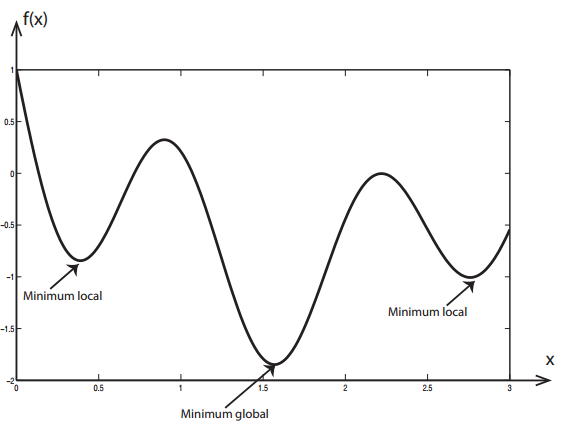
\includegraphics[width=0.6\textwidth,keepaspectratio]{diff_optGlobal_optLocal}
	\caption[Différence entre un optimum global et un optimum local]{Différence entre un optimum global et un optimum local \cite{boussaid}}
\end{figure}

Les fonctions objectifs peuvent être continues, discontinues,
linéaires, non-linéaires, convexes, non-convexes, uni-modales,
multi-modales, séparables ou non-séparables\cite{Momin_Yang_2013}.

\begin{itemize}
	\item La séparabilité mesure la difficulté d'une fonction. En général, une fonction séparable est plus ou moins facile à minimiser en la comparant avec une autre non-séparable car chaque variable d'une fonction séparable est indépendante des autres. Du coup, la fonction peut être écrite sous forme d'une somme de plusieurs fonctions, chacune à une seule variable\cite{Momin_Yang_2013}.
	\item Le nombre de pics dans le graphe d'une fonction correspond à sa modalité. Une fonction multi-modale est une fonction qui admet plusieurs optimums locaux. Ce type de fonctions est difficile à minimiser car l'algorithme peut stagner dans un optimum local et ne plus en sortir. 
	\item La difficulté d'un problème augmente avec l'augmentation de sa dimension, ce qui représente une barrière pour la plupart des algorithmes d'optimisation. 
\end{itemize}

Les classes des problèmes d'optimisation continue sont variées, d'où la difficulté de trouver une méthode de résolution générale efficiente. C'est la raison pour laquelle nous nous intéressons dans ce travail aux problèmes d'optimisation continue mono-objectif, sans contraintes et de minimisation.

A l'augmentation de la taille du problème, ce dernier devient plus difficile à résoudre et ne peut pas être résolu de manière exacte dans un temps raisonnable, d'où l'intérêt des méthodes approchées qui évitent l'explosion combinatoire par l'exploration partielle de l'espace de recherche mais d'une manière intelligente.\\

\section{Les méta-heuristiques}

Ce sont des algorithmes génériques qui utilisent des
heuristiques pour donner des solutions approchées à des problèmes
complexes en utilisant une approche guidée par une technique
spécifique.

Les méta-heuristiques se présentent sous deux catégories, celles qui
ne sont pas bio-inspirées telles que la recherche Tabou et la recherche
dispersée, et celles qui le sont telles que l’algorithme génétique et les
algorithmes issus de l’intelligence en essaim (par exemple les algorithmes des
colonies de fourmis et d'essaims d’abeilles qui ont été initialement
conçus pour des problèmes combinatoires et aussi les algorithmes Bat Algorithm (BA) et Particle Swarm Optimization (PSO) qui ont été développés pour des problèmes continus).

Toutes les méta-heuristiques comportent deux stratégies de
recherche :

\begin{itemize}
	\item l'intensification par recherche locale dans une seule région de l'espace de recherche,
	\item la diversification qui consiste à changer de région pour en explorer d'autres.
\end{itemize}

L'importance de la stratégie de recherche varie d'une méta-heuristique à une autre, cela dépend généralement des besoins souhaités:

\begin{itemize}
	\item plus d'intensification mène à une solution de meilleure qualité,
	\item plus de diversification mène à trouver une solution en un temps plus réduit,
	\item un compromis entre les deux mène à une meilleure solution en un temps plus réduit.
\end{itemize}

\section{L'intelligence en essaim}

C'est une technologie très importante de l'intelligence artificielle qui recouvre un ensemble d'algorithmes à base de population d'agents simples. Un algorithme issu de l'intelligence en essaim se base sur deux principes:

\begin{itemize}
	\item l'observation à partir des phénomènes naturels intelligents et plus précisément des comportements en groupe,
	\item la simulation des comportements collectifs des insectes (fourmis
	et abeilles) et des animaux (poissons et oiseaux) qui traduisent une intelligence collective.
\end{itemize}

Un essaim peut être vu comme étant un groupe d'agents où chacun
fait une tâche élémentaire. L'efficacité de l'essaim peut être remarquée
d'un point de vue global qui est établi grâce à l'interaction sociale entre les
agents. Cette interaction influence les comportements individuels
des agents et les pousse à apporter leur contribution pour atteindre ensemble un but global qui représente le but de l'essaim.

L'intelligence en essaim a été appliquée à plusieurs domaines:

\begin{itemize}
	\item l'optimisation combinatoire (voyageur de commerce,
	ordonnancement et planification, transport moderne,
	télécommunications, etc...),
	\item l'optimisation continue (optimisation des fonctions numériques),
	\item les applications de l'intelligence artificielle (traitement automatique
	du langage, traitement d'image et robotique),
	\item les applications de divertissement (films et jeux vidéo),
	\item la fouille de données (Data Mining),
	\item le routage dans les réseaux,
	\item les applications Web (recherche, filtrage et sécurité).
\end{itemize}

\section*{Conclusion}

Après avoir introduit le domaine de l'intelligence artificielle et plus particulièrement celui de l'optimisation, nous avons abordé la différence entre l'optimisation combinatoire et celle continue. Puis, nous avons présenté la philosophie des méta-heuristiques et de l'intelligence en essaim ainsi que ses différentes adaptations. Le chapitre suivant est consacré aux travaux réalisés par les chercheurs dans le domaine de l'optimisation continue.

	\chapter{L'optimisation continue} 

\section*{Introduction}

Avant de pouvoir proposer n'importe quel algorithme d'optimisation continue, il faudra d'abord établir une étude comparative entre les différentes approches proposées dans le passé. Cela permet d'élargir notre champ de connaissances en tenant compte des points forts des autres algorithmes et de ne pas reprendre les erreurs commises par les autres chercheurs.

Nous ne pouvons pas présenter toutes les approches proposées auparavant, donc nous nous contentons de le faire pour quelques méta-heuristiques et les domaines dans lesquelles elles ont été appliquées pour l'optimisation continue.
\section{Méta-heuristiques pour les problèmes à variables continues}
\subsection{L'algorithme Particle Swarm Optimization (PSO)}
C'est en 1995 que l'algorithme PSO a été proposé par Kennedy et Eberhart pour traiter les problèmes d'optimisation continue \cite{KENNEDY_EBERHART_1995}.

Cette approche simule les comportements des particules telles que les poissons et les oiseaux migrateurs qui se comportent en fonction du comportement global du groupe.

Du point de vu informatique, les particules représentent les solutions candidates d'une population. Les particules évoluent simultanément par partage d'information avec le voisinage. Le rôle de chaque particule est de générer une solution en se basant sur son vecteur vitesse, puis de chercher à améliorer sa position dans l'espace en modifiant son vecteur vitesse à l'instant $t+1$ grâce à trois critères qui caractérisent son mouvement: \\
\vspace{-2em}

\begin{itemize}
	\item sa propre vitesse à l'instant $t$,
	\item sa meilleure position par le passé,
	\item la meilleure position connue de la population.
\end{itemize}

Il y a trois types de comportements de particules:

\begin{itemize}
	\item égoïste (la particule prend son propre chemin),
	\item conservatif (la particule conserve sa position),
	\item panurgique (la particule suit le meilleur comportement du groupe).\\
\end{itemize}

L'algorithme PSO est le suivant.\bigskip

\begin{algorithm}[H]
	\caption{PSO}
	\KwIn{La condition d'arrêt}
	\KwOut{La meilleure solution trouvée}
  	\Begin{
		Initialisation aléatoire de l'essaim de particules\;
		\While{la condition d'arrêt est non vérifiée}
		{
			$gbest \leftarrow$ meilleur $pbest_i$ de toutes les particules\;
			\For{chaque particule$_i$}
			{
				$v_i^{t+1}\leftarrow w v_i^t + r_1 c_1 (x_i - pbest_i)+r_2 c_2(x_i - gbest)$\;
				Mise à jour de la position de la particule $x_i^{t+1} \leftarrow x_i^t + v_i^{t+1}$\;
			}
			\For{chaque particule$_i$}
			{
				Calculer la valeur de la fonction $fitness$\;
				\If{$fitness < pbest_i$ \tcc{meilleure valeur rencontrée pour la particule}}{
					$pbest_i \leftarrow fitness$\; 
				}
			}
  }
}
\end{algorithm}

\parbox[c][7em][s]{\textwidth}{}

\begin{spacing}{1.6}

PSO a été également développé et appliqué sur un problème de reconfiguration des systèmes de
distribution pour minimiser la perte d'énergie. La méthode proposée
reformule le problème en tant que problème d'optimisation non linéaire.
Elle a été examinée et testée sur les systèmes de test standards IEEE14,
IEEE30 et IEEE118 \cite{esmin2012application}.

\bigskip

Encore, PSO a été appliqué sur un problème de modélisation des
réseaux de transport pour minimiser le temps de voyage tout en
assurant que le budget n'excède pas une certaine limite. PSO a été
comparé avec l'algorithme Hybridized Ant Colony Optimization (HACO) qui a été conçu spécialement pour ce genre de problèmes et a donné de bons résultats \cite{babazadeh2011application}.

\bigskip

Malheureusement, PSO souffre du problème de la convergence prématurée, c'est la raison pour laquelle une version mathématique intégrale modifiée de PSO a été mise au point pour le problème de planification des systèmes de chauffage afin de minimiser le coût du système pour un
cycle de vie donné. Il a été prouvé que la version améliorée de PSO
(improved PSO, IPSO) résout le problème efficacement et fournit des
informations qui montrent qu'il est apte à régler des problèmes de
planification réels \cite{ma2013application}.

\bigskip

\subsection{L'algorithme Bat Algorithm (BA)}
C'est un algorithme bio-inspiré récent, développé par Xin-She Yang en 2010 \cite{yang2010new} pour les problèmes d'optimisation globale. Il est inspiré des écholocations naturelles des chauves-souris qui peuvent trouver et discriminer les différents types d’insectes et éviter les obstacles, même
dans l’obscurité totale.

\bigskip

Cet algorithme se base sur les trois étapes répétitives suivantes:

\bigskip
\begin{itemize}
	\item l'évaluation de la performance de chaque chauve-souris,
	\item la mise à jour des meilleures solutions locales et globales,
	\item la mise à jour de la position, de la vitesse et de la fréquence de chaque chauve-souris. 
\end{itemize}

\end{spacing}

\vspace{-5em}
L'algorithme BA est le suivant.

\bigskip\bigskip

\begin{algorithm}[H]
	\KwIn{Les paramètres de l'algorithme et la condition d'arrêt}
	\KwOut{La meilleure solution trouvée}
	\Begin{
			Définir la fonction objectif $f(x),x=(x_1,...,x_d)^T$\;
			Initialiser la population des chauves-souris $x_i(i=1,2,...,n)$ et la vitesse de chacune des chauves-souris $v_i$\;
			Calculer la fréquence d'impulsion $f_i$ à la position $x_i$\;
			Initialiser les taux d’émissions de pulsation $ri$ et l'intensité $A_i$\;
			\While{$t$ < nombre maximum des itérations}
			{
				Générer de nouvelles solutions par l’ajustement des fréquences,
				et mettre à jour les vitesses et les positions\;
				\If{$rand>r_i$}
				{
					Sélectionner une solution parmi les meilleures solutions\;
					Générer une solution locale autour de la meilleure solution sélectionnée\;
				}
				Générer une nouvelle solution en volant aléatoirement\;
				\If{$rand<A_i$ et $f(x_i)<f(x_*)$}
				{
					Accepter les nouvelles solutions\;
					Incrémenter $r_i$ et réduire $A_i$\;
				}
				Classer les chauves-souris et trouver la meilleure solution courante\;
			}
			Post-traitement des résultats et visualisation\;		
		}
	\caption{BA}
\end{algorithm}

\vspace{3em}
\begin{spacing}{1.6}
La mise à jour des vitesses et des positions des chauves-souris est similaire à celle des particules dans l'algorithme PSO. C'est pour cela que BA est considéré comme une extension de PSO avec une recherche locale contrôlée par l'intensité et par le taux d'émission des ondes.
\end{spacing}

\section{Méta-heuristiques adaptées aux problèmes à \\ \mbox{variables} continues}
\subsection{L'algorithme Ant Colony Optimization pour les domaines continus (ACO$_\mathbb{R}$)}
Initialement proposée en 1991 \cite{dorigo2006ant}, l'approche ACO s'inspire du comportement naturel des fourmis. Ces insectes commencent par une exploration aléatoire de l'espace de recherche, puis déposent de la phéromone en fonction de la quantité et de la qualité de nourriture trouvée. Après une certaine période de temps, la meilleure source de nourriture aura la plus forte concentration de phéromone. Du coup, la colonie de fourmis s'y dirige.

En informatique, l'approche ACO se base sur la construction incrémentale (variable par variable) des solutions. L'ensemble des composants possibles de la solution est défini par le problème. 

A chaque étape de construction, une fourmi fait un
choix probabiliste pour choisir le prochain composant $c_{ij}$ de la solution à
partir de l'ensemble des composants admissibles $N(s^p)$. La règle exacte de ce choix probabiliste varie d'un algorithme à un autre, la meilleure connue est celle de Ant System (AS) \cite{dorigo1996ant}:

$$ p(c_{ij}|s^p) = \frac{\tau^\alpha_{ij}\cdot\eta(c_ij)^\beta}{\sum_{c_{il} \in N(s^p)} \tau^\alpha_{il}\cdot\eta(c_ij)^\beta} \forall c_{ij} \in N(s^P),
$$

où:
\begin{itemize}
	\item $t_{ij}$ est la valeur de phéromone associée au composant $c_{ij}$,
	\item $\eta$ est la fonction de pondération qui associe, à chaque étape de
	construction, une valeur heuristique à chaque composant admissible
	de la solution $c_{ij} \in N(s^P)$,
	\item $\alpha$ et $\beta$ sont des paramètres positifs qui déterminent la relation entre
	l'information de phéromone et l'information heuristique.
\end{itemize}
\bigskip\bigskip
Une extension de l'approche des colonies de fourmis, appelée ACO$_\mathbb{R}$,  a été présentée pour les domaines continus \cite{SOCHA_DORIGO_2006} . 

Dans l'algorithme ACO$_\mathbb{R}$, Socha et Dorigo proposent d'utiliser une distribution de
probabilité continue (qui est une fonction de densité de probabilité,
Probability density function en anglais, PDF) au lieu d'utiliser une distribution de
probabilité discrète dans le processus de décision.

Dans ACO$_\mathbb{R}$, au lieu de choisir un composant $c_{ij}\in N(s^p)$, une fourmi
échantillonne une PDF en utilisant un ensemble de solutions appelé
archive de solutions. Cette archive remplace la table de phéromone dans l'approche ACO combinatoire, et la mise à jour de la phéromone se traduit ici par le rajout et le retrait des solutions de cette archive. 

Initialement, l'archive de solutions contient $k$ solutions
aléatoires ($k$ est un paramètre empirique). Ensuite, à chaque itération, $m$ nouvelles solutions sont
générées, évaluées et ajoutées à l'archive qui sera donc de taille $k+m$ ($m$
étant le nombre de fourmis). L'archive est par la suite triée selon les
qualités des solutions et seulement les $k$ meilleures sont gardées (la taille
de l'archive restera égale à $k$ à la fin de chaque itération).\\

La représentation de l'archive est la suivante:

\begin{figure}[H]
	\centering
	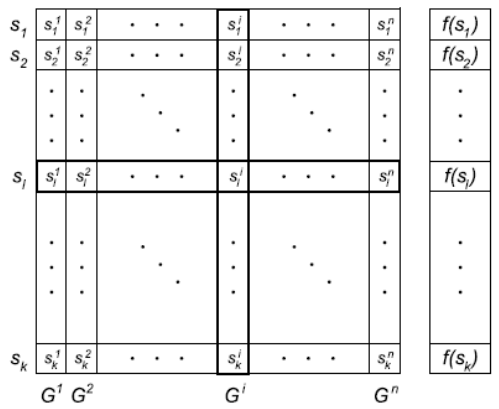
\includegraphics[width=0.65\textwidth,keepaspectratio]{archive}
	\caption{Archive des solutions dans l'algorithme ACO$_\mathbb{R}$}
\end{figure}


\begin{itemize}
	\item $n$ est la taille de la solution (dimension de la fonction problème),
	\item $k$ est le nombre de solutions dans l'archive,
	\item $s^i_l$ est le $i^{ème}$ composant de la $l^{ème}$ solution.
\end{itemize}

Chaque ligne de l'archive correspond à une solution construite par une fourmi. La
qualité de chaque solution est calculée par la fonction objectif et stockée
dans l'archive.

Socha et Dorigo utilisent une fonction de densité de probabilité unidimensionnelle (à une seule variable) et multi-modale basée sur une fonction gaussienne noyau qui représente une somme pondérée de plusieurs fonctions gaussiennes $g^i_l$  où $l$ est l'indice de la solution et $i$ est l'indice du composant. La fonction gaussienne noyau est définie comme suit:

$$
G^i (x) = \sum^{k}_{l=1} \omega_l g_l^i(x) = \sum^{k}_{l=1} \omega_l \frac{1}{\sigma^i_l \sqrt{2\pi}} \mathrm{e}^{-\frac{(x-\mu^i_l)^2}{2\sigma_l^{i^2}}}
,$$

où:
\begin{itemize}
	\item $l \in$ $\{1,...,k\}$,
	\item $i \in$ $\{1,...,n\}$,
	\item $w_l$ est le poids de la $l^{ème}$ solution.
\end{itemize}


Le poids de chaque fonction est calculé selon la fonction gaussienne suivante:

$$
\omega_l = \frac{1}{qk\sqrt{2\pi}} \textrm{e}^{-\frac{(l-1)^2}{2q^2 k^2}}.
$$

Cette formule définit le poids comme étant une valeur de la fonction
gaussienne avec argument $l$, moyenne $\mu=1$ et variance $\sigma=qk$,  où $q$ est un paramètre empirique de l'algorithme.

Lorsque $q$ est petit, les meilleures solutions sont fortement préférées et lorsqu'il est grand, la probabilité devient plus uniforme.

En pratique, dans le processus de construction de solution, chaque composant de la nouvelle solution est traité indépendamment des autres.
Chaque fourmi choisit une des solutions de l'archive selon son poids. La probabilité $p_l$ de choisir la $l^{ème}$ solution est donnée par:
$$
p_l = \frac{\omega_l}{\sum_{r=1}^{k} \omega_r}.
$$

Ensuite, à l'étape $i$, l'algorithme échantillonne la fonction gaussienne associée au $i^{ème}$ composant de la solution choisie en utilisant une fonction
de densité de probabilité gaussienne, avec $\mu^i_l=s^i_l$ et $\sigma^i_l$ donnée par:
$$
\sigma_l^i = \xi \sum_{e=1}^{k} \frac{|S_e^i - S_l^i|}{k-1}.
$$

Cette formule représente la distance moyenne entre la $i^{ème}$ variable de la $l^{ème}$ solution
(solution choisie) et la $i^{ème}$ variable des autres solutions de l'archive,
multipliée par un paramètre $\xi$.

Ce paramètre a un effet similaire à celui du taux d'évaporation de la phéromone dans l'approche ACO. Plus $\xi$ est grand, plus la vitesse de convergence de l'algorithme est petite.

Après le calcul de $\mu^i_l$ et $\sigma^i_l$, la $i^{ème}$ variable de la nouvelle solution aura comme valeur un nombre aléatoire généré en obéissant à la loi gaussienne $N(\mu^i_l,\sigma^i_l)$.  

Le processus de construction de solution est répété $m$ fois pour chaque
dimension $i=1,...,n$ du problème. Après chaque construction de solution, la mise à jour
de la phéromone est traduite par le fait d'ajouter $m$ nouvelles solutions
générées à l'archive $T$ et d'éliminer le même nombre de plus mauvaises solutions; on garde donc le même nombre $k$ de solutions dans l'archive. Ce
processus permet de ne garder que les $k$ meilleures solutions, ce qui va
permettre de bien guider les fourmis dans leur processus de recherche.

L'algorithme ACO$_\mathbb{R}$ permet d'ajouter des activités qu'une simple
fourmi ne peut pas faire: recherche locale sur les solutions construites, récolte d'une information globale pour décider s'il est utile de déposer
encore de la phéromone, etc... Cependant, ces activités n'ont pas été appliquées par Socha et Dorigo.

Le pseudo code de l'algorithme ACO$_\mathbb{R}$ est donné comme suit:\\

\begin{algorithm}[H]
	\KwIn{$k$,$m$,$n$,$q$,$\xi$ et la condition d'arrêt}
	\KwOut{La meilleure solution trouvée}
	\Begin{
	Initialiser et évaluer $k$ solutions\;
	\tcp{Trier les solutions et les mettre dans l'archive}
	$T = Trier(S_1 ... S_{k})$\;
	\While{la condition d'arrêt est non vérifiée}{
		\tcp{Générer $m$ nouvelles solutions}
		\For{$l=1$ \KwTo $m$}{
			\tcp{Construire une solution}
			\For{$i=1$ \KwTo $n$}{
				Choisir une fonction gaussienne $g^i_j$ selon les poids\;
				Échantillonner la fonction $g^i_j$ avec le paramètre $\mu^i_j \cdot \sigma^i_j$\;
			}
			Sauvegarder et évaluer la solution générée\;
		}
		\tcp{Trier les solutions et choisir les $k$ meilleures}
		$T = Meilleure(Trier(S_1 ... S_{k+m}),k)$\;
	}
}
\caption{ACO$_\mathbb{R}$}
\end{algorithm}



\subsection{L'algorithme ACO$_\mathbb{R}$ avec la théorie des perspectives (\mbox{ACO$_\mathbb{R}$-PT})}
Riadi Indra \cite{riadi2014cognitive} a proposé une amélioration de l'algorithme ACO$_\mathbb{R}$ qui garde le même principe que celui de ACO$_\mathbb{R}$ sauf qu'elle modifie la transition d'état lors de la phase de construction. Une solution n'est pas choisie en se basant sur son poids seulement, mais aussi sur son évaluation. C'est pourquoi Indra commence par calculer un point de référence qui est la moyenne des évaluations des solutions de l'archive.

$$point~de~référence = moyenne (f(s_1),f(s_2),...,f(s_k)).$$

Ensuite, il commence à séparer les solutions de l'archive en deux groupes. Les solutions qui ont une évaluation plus petite que celle du point de référence auront un gain négatif par rapport à l'écart du point de référence et les solutions qui ont une évaluation plus grande ou égale à celle du point de référence auront un gain positif.

De plus, une valeur probabiliste est calculée pour chaque solution. Le nouveau poids (perspective) de la solution est obtenu par la multiplication de son gain par sa valeur probabiliste.

La meilleure solution est celle qui a le poids le plus élevé et qui va donc être utilisée pour calculer la nouvelle valeur de phéromone.

\subsection{L'algorithme Continuous Ant Colony Optimization (CACO)}

Cet algorithme, développé par Bilchev et Parmee \cite{bilchev1995ant}, représente le premier essai pour adapter un algorithme inspiré du comportement des fourmis aux problèmes d'optimisation continue. Dans CACO, les fourmis commencent à partir d'un point appelé $nid$, situé quelque part dans l'espace de recherche. Les bonnes solutions trouvées sont stockées en tant qu'ensemble de vecteurs et proviennent du nid. A chaque itération, les fourmis font un choix probabiliste sur un des vecteurs. Ensuite, elles continuent la recherche à partir du vecteur choisi en faisant des mouvements aléatoires. Les vecteurs sont mis à jour par les meilleurs résultats trouvés. 

Bien que les auteurs de CACO prétendent qu'ils se sont inspirés de l'approche ACO originale, CACO présente plusieurs différences avec ACO. En effet, la notion de $nid$ n'existe pas dans l'approche ACO. De plus, CACO ne fait pas une construction incrémentale des solutions alors que celle-ci est l'une des caractéristiques principales de ACO. Donc, CACO n'est pas une extension de ACO.  

\subsection{L'algorithme Continuous Interacting Ant Colony (CIAC)}

Cette approche, basée sur le comportement des fourmis, a été présentée par Dréo et Siarry \cite{dreo2004continuous}. CIAC utilise deux types d'interaction entre les fourmis, l'information stigmergique (points de phéromone déposés dans l'espace de recherche) et la communication directe entre les fourmis. Ces dernières font des mouvements stratégiques en suivant la phéromone et en communicant entre elles. De même que CACO, CIAC n'est pas une extension de ACO car il ne construit pas les solutions de façon incrémentale et est basé sur une communication directe entre les fourmis.

\subsection{L'algorithme Taboo Search (TS)}
La première adaptation de la recherche Tabou aux domaines continus est présentée par Cvijovic et Klinowski en 1995 \cite{cvijovic1995taboo}. Dans cet algorithme, les auteurs ont introduit une structure de voisinage pour l'espace continu qu'ils ont appelée \emph{voisinage conditionnel}. L'espace de solutions $S$ (qui représente un hyper-cube dans $\mathbb{R}^n$, où n est le nombre de variables) est partitionné en des cellules disjointes en divisant en $p_1, p_2,...,p_n$ partitions, les intervalles de coordonnées au long des axes $x_1, x_2,...,x_n$ .

A chaque itération, $n_s$ points sont tirés à partir de $n_c$ partitions choisies au hasard en utilisant une distribution uniforme. Ces points vont constituer les voisins de la solution courante $s^*$. La taille du voisinage $N(s^*)$ est égale à $n_c n_s$.

\subsection{L'algorithme Continuous Tabu Search (CTS)}
Une autre extension de la recherche Tabou proposée par Siarry et Berthiau \cite{siarry1997fitting} explore la notion de voisinage inventée par N. Hu \cite{Hu_1992} qui se base sur le principe de disques centrés par la solution.

\begin{figure}[H]
	\centering
	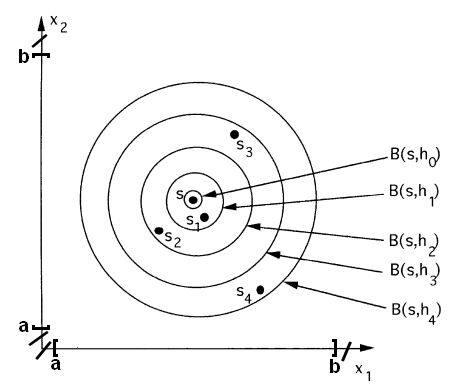
\includegraphics[width=0.45\textwidth,keepaspectratio]{partitionnement_voisinage}
	\caption{Partitionnement du voisinage d'une solution dans CTS}
\end{figure}

Les voisins de la solution sont pris chacun d'une couronne qui sépare les frontières de deux disques consécutifs. Une explication détaillée de cette notion sera expliquée dans le prochain chapitre.

CTS commence à partir d'une solution aléatoire, puis génère un certain nombre fixe de voisins et continue avec le meilleur voisin, même si son évaluation est pire que celle de la solution courante (voisinage en anneau).

Pour éviter de boucler sur les mêmes voisins, chaque voisin généré est inséré dans une liste Tabou circulaire qui garde trace des dernières solutions rencontrées vers lesquelles nous ne devons pas revenir. Cependant, ce processus risque de contourner des mouvements utiles, ce qui nécessite l'incorporation d'un mécanisme d'aspiration qui permet d'éviter une telle situation.  

L'algorithme s'arrête lorsqu'il trouve l'optimum ou lorsqu'il n'arrive pas à améliorer la solution au bout d'un certain nombre d'itérations.
 
\subsection{L'algorithme Enhanced Continuous Tabu Search (ECTS)}
C'est une adaptation de la recherche Tabou aux domaines continus qui consiste d'abord à faire une diversification pour détecter les régions prometteuses, puis à effectuer une intensification afin de trouver l'optimum dans la région la plus prometteuse \cite{Chelouadh_siarry_2001} .

Le voisinage est défini de la même manière que dans CTS sauf que les auteurs ici considèrent des hyper-rectangles au lieu des disques. 

L'algorithme ECTS est le suivant:\\

\begin{algorithm}[H]
	\KwIn{Les paramètres de l'algorithme et la condition d'arrêt}
	\KwOut{La meilleure solution trouvée}
	\Begin{
		Diversification\; 
		Chercher la région la plus prometteuse\;
		\While{la condition d'arrêt est non vérifiée}{
			Intensification\;
			Mise à jour de la meilleure solution\;
		}
	}
	\caption{ECTS}
\end{algorithm}
\bigskip

\subsection{L'algorithme Continuous Reactive Tabu Search (CRTS)}
\begin{spacing}{1.4}
Une amélioration de la recherche Tabou pour les domaines continus a été proposée par Battiti et Tecchiolli \cite{battiti1996continuous}, et qui s'inspire de l'approche combinatoire Reactive Tabu Search (RTS) en la combinant avec un minimisateur stochastique. Le composant combinatoire sert à localiser les régions prometteuses (qu'ils ont appelées boîtes) à partir desquelles le minimisateur effectue sa recherche locale. La taille des boîtes ainsi que les paramètres de recherche sont adaptés automatiquement à la structure locale de la fonction objectif.\\[2em]
\end{spacing}

Les auteurs ont développé une fonction d'évaluation des boîtes qui permet d'indiquer si la boîte contient de bonnes solutions. Ils ont testé deux méthodes de calcul et ont exprimé chacune dans un algorithme:
\begin{itemize}
	\item CRTS$_{average}$ (CRTS$_{ave}$) qui considère la moyenne des évaluations des solutions dans la boîte:
	$$X_i: f(B)\equiv \left(\frac{1}{N_B}\right)\sum_{i=1}^{N_B}f(X_i),$$ où $N_B$ est le nombre de points.
	\item CRTS$_{minimum}$ (CRTS$_{min}$) qui considère le minimum des évaluations des solutions dans la boîte:
	$$f(B)\equiv min_{i\in(1,...,N_B)} f(X_i).$$
\end{itemize}


\subsection{L'algorithme Continuous Genetic Algorithm (CGA)}
L'algorithme génétique se base sur les opérateurs suivants:

\begin{itemize}
	\item la sélection des individus qui doivent se reproduire par la technique de tirage à roulette ou par tournoi ou par rang,
	\item le croisement des individus sélectionnés,
	\item la mutation (modification aléatoire) des nouveaux individus,
	\item le remplacement des parents par les nouveaux individus.
\end{itemize}

La nouvelle population sera construite des meilleures individus de la population courante.
 
La version continue de l'algorithme génétique redéfinit les opérateurs de croisement et de mutation en tenant compte de la taille et de la distribution de la population dans l'espace de recherche \cite{Chelouadh_siarry_2000}.

La taille de la population est initialement large pour une meilleure convergence de l'algorithme, mais elle sera réduite au fur et à mesure pour éviter une explosion en termes de temps d'exécution. De plus, pour une meilleure exploration de l'espace de recherche, la population initiale est construite par des solutions suffisamment éloignées les unes des autres et une solution n'est choisie que lorsqu'elle n'appartient à aucun voisinage des autres solutions de la population.

Les auteurs, comme N. Hu\cite{Hu_1992}, utilisent le principe de disque pour explorer le voisinage d'une solution.

L'algorithme CGA est le suivant:\\

\begin{algorithm}[H]
	\KwIn{La condition de convergence}
	\KwOut{La meilleure solution trouvée}
	\Begin{
		Définir la fonction coût, le coût et les variables\;
		Choisir les paramètres de l'algorithme\;
		\While{la condition de convergence est non vérifiée}{
			Choisir les parents\;
			Croisement\;
			Mutation\;
		}
	}
	\caption{CGA}
\end{algorithm}

\subsection{L'algorithme Enhanced Simulated Annealing (ESA)}
Cet algorithme développé par Siarry et ses camarades \cite{siarry1997enhanced}, manipule les problèmes de grande taille en faisant une discrétisation des variables. La recherche aléatoire itérative est remplacée ici par une exploration de plusieurs espaces euclidiens.

\vspace{1em}

Cet algorithme a été prouvé efficace pour résoudre les problèmes de taille 2 à 200 variables. 

\subsection{L'algorithme Evolutionary Strategies (ES)}
Différentes adaptations de l'algorithme évolutionniste ES aux domaines continus ont vu le jour à travers les années.
\begin{itemize}
	\item (1+1)ES \cite{kern2004learning} se base sur un seul parent qui génère une progéniture par itération. Seul l'individu représentant la meilleure solution est gardé.
	\item Cumulative Step Size Adaptation (CSA-ES) \cite{hansen2003reducing} contrôle la taille du pas global en utilisant un chemin traversé par la population parente à travers un certain nombre de générations,
	\item Covariance Matrix Adaptation (CMA-ES) \cite{hansen2003reducing} est une variante de CSA-ES avec une adaptation aléatoire de la matrice de covariances.
	
\end{itemize}

\subsection{L'algorithme Iterated Estimation of Distribution \\Algorithm (IDEA)}
C'est une adaptation de Estimation of Distribution Algorithms (EDAs) pour les problèmes d'optimisation continue, développée par Bosman et Thierens en 2002 \cite{bosman2002multi}. Pour estimer la distribution de la population parente, IDEA exploite le fait que chaque probabilité jointe multi-variée peut être exprimée en tant que factorisation conditionnelle:
$$
P(x_i,...,x_n)=\prod_{i=1}^{n}P(x_i|x_{i+1},x_{i+2},...,x_n).
$$

Le modèle probabiliste de la population parente est reconstruit à chaque itération.

\subsection{L'algorithme Mixed Bayesian Optimization Algorithm  (MBOA)}
Cet algorithme développé par Ocenasek et Schwarz \cite{ocenasek2002estimation}, est basé sur un réseau bayésien avec des structures locales sous forme d'arbres de décision qui capturent les dépendances mutuelles entre les individus parents. MBOA est une extension continue de l'algorithme hierarchical BOA initialement conçu pour le domaine binaire. MBOA peut traiter les variables de type mixte (discret et continu).

\subsection{L'algorithme INTEROPT}
C'est une méthode numérique conçue par Bilbro Griff et Snyder Wesley  \cite{bilbro1991optimization}, pour optimiser les fonctions non-convexes. Elle est basée principalement sur l'approche du recuit simulé mais traite les problèmes à variables continues. La méthode est complètement générale et capable de résoudre les problèmes qui ont une grande taille.

\vspace{-1em}

\section*{Conclusion}
Chaque méta-heuristique a ses avantages et ses inconvénients. La stratégie de recherche diffère d'un algorithme à un autre mais le but est toujours le même, c'est d'essayer d'arriver à la meilleure solution au problème dans les meilleurs délais possibles.
 
Nous avons présenté deux catégories de méta-heuristiques, celles conçues pour des problèmes à variables continues et celles développées à l'origine pour des problèmes à variables discrètes et qui ont été transformées pour s'adapter aux problèmes à variables continues. Le chapitre suivant est consacré à l'algorithme Bee Swarm Optimization (BSO) et à notre propre adaptation de ce dernier aux problèmes d'optimisation continue.


	\chapter {Adaptation de BSO aux problèmes d'optimisation continue}

\section* {Introduction}
L'objectif de notre travail est d'adapter la méta-heuristique BSO aux problèmes d'optimisation continue sans trop affecter sa structure initiale. Après un rappel du principe général de BSO, nous passons en revue les domaines dans lesquels elle a été appliquée. Puis, nous exposons notre contribution qui consiste à son adaptation à l'optimisation continue.

\section{L'algorithme Bee Swarm Optimization (BSO)}

\subsection{Principe}

L’algorithme BSO classique s’inspire du comportement naturel des essaims
d'abeilles.

L'abeille éclaireuse quitte la ruche à la recherche du nectar. Quand
elle le trouve, elle revient à la ruche avec un peu de récolte, puis elle fait une danse circulaire. Pour les sources de nourriture qui sont loin de la ruche, l'abeille éclaireuse change petit à petit sa danse en une danse en huit (la danse d'abeille est riche en informations parce qu'elle indique la
quantité de la nourriture trouvée, la distance qui la sépare de la ruche et la direction de sa source).

L'essaim d'abeilles se dirige vers la source de nourriture la plus riche,
même si elle est la plus éloignée (ce comportement a été confirmé par
l'expérience de Seeley et ses camarades \cite{seeley1991collective}).

Du point de vue informatique, on associe à l'abeille
éclaireuse un sommet de référence qui est une solution construite
aléatoirement ou en suivant une heuristique. A partir de ce sommet, on
génère $n$ autres solutions en utilisant le paramètre $Flip$ permettant de déterminer un ensemble de points de l'espace de recherche à explorer. L’ensemble de
ces solutions définit la zone de recherche.

Ensuite, on attribue chaque point ou solution de la zone de recherche à une abeille, qui fera une recherche locale afin d’aboutir à un optimum local. L'ensemble des optimums locaux est mis dans une table appelée $Danse$. Le meilleur optimum local à une itération sera considéré comme le nouveau sommet de référence de la prochaine itération.

Pour éviter de boucler indéfiniment dans la même zone de
l’espace de recherche, le sommet de référence est sauvegardé à chaque
fois dans une liste appelée $Tabou$.

Dans un premier temps, le choix du sommet de référence est fait en
se basant sur les qualités des solutions (phase d’intensification). Puis, si après
une certaine période de temps, on n'arrive pas à améliorer la solution, on
utilise le critère de diversité pour changer de région et en explorer d’autres (phase de diversification).\\

L’algorithme BSO est le suivant:

\begin{algorithm}
	\caption{BSO}
	\KwIn{Les paramètres de l'algorithme et la condition d'arrêt}
	\KwOut{La meilleure solution trouvée}
	\Begin{
    Soit $Sref$ la solution trouvée par l'abeille éclaireuse\;
    \While{la condition d'arrêt est non vérifiée}{
      Insérer $Sref$ dans la liste $Tabou$\;
      Déterminer la zone de recherche à partir de $Sref$\;
      Attribuer une solution $s$ de la zone de recherche à chaque abeille\;
      \For{chaque abeille}{
        Recherche locale avec la solution $s$\;
        Mettre l'optimum local dans la table $Danse$\;
      }
      Choisir le nouveau sommet de référence $Sref$\;
    }
  }
\end{algorithm}

\subsection{Applications}

C'est en 2005 que l’algorithme BSO a été proposé et appliqué sur le problème de satisfiabilité MAXW-SAT puis adapté à plusieurs domaines d’application parmi lesquelles la fouille de données et la recherche d’information \cite{DRIAS_SADEG_YAHI_2005}.

Une méthode hybride a été proposée pour prendre en charge les instances volumineuses du problème SAT.
Cette méthode se base essentiellement sur la méta-heuristique bio-inspirée BSO et sur le paradigme multi-niveaux. Dans ce travail, on perçoit l’importance de la combinaison de deux approches prometteuses afin de bénéficier de leurs avantages \cite{DJEFFAL_DRIAS_2013}.

Une combinaison entre le Clustering (une tâche du Data Mining) et la méta-heuristique BSO a été mise au point pour améliorer l’efficacité de la résolution du problème
SAT. L’approche suivie consiste à explorer judicieusement l’espace de
recherche avant de lancer le processus de recherche de solutions qui va
réduire la complexité des instances volumineuses du problème SAT. Deux
méthodes ont été proposées. La première consiste à intégrer le Clustering
dans la structure originale de BSO, qui va mener à suggérer une version
avancée de BSO. La deuxième méthode consiste à faire un Clustering sur
les données avant de lancer BSO. Cette manière de procéder aide à
réduire le nombre de clauses et le nombre de variables des instances SAT
et donc le temps d'exécution \cite{DRIAS_DOUIB_HIRECHE_2013}.

D'autres auteurs ont proposé un nouvel algorithme de
recherche de règles d'association basé sur une version améliorée de BSO
avec trois heuristiques différentes pour explorer l'espace de recherche.
Cette approche a été implémentée et testée sur différentes bases de
données de petite, moyenne et grande taille. Les résultats obtenus
montrent que l'approche proposée est meilleure que certains algorithmes
de la littérature en termes de qualité et de temps d'exécution \cite{DJENOURI_DRIAS_HABBAS_2014}.

Nous nous intéressons dans ce travail à l'adaptation de BSO aux problèmes d'optimisation continue afin d'élargir son champ d'application. Nous allons présenter notre contribution à cette problématique en développant une version de BSO pour les problèmes à variables continues, que nous avons appelée Continuous Bee Swarm Optimization (CBSO).

\section{Continuous Bee Swarm Optimization (CBSO)}
Le problème que nous traitons consiste en des fonctions
mathématiques à plusieurs dimensions (variables). A noter que la fonction problème est elle-même la fonction objectif qu'on cherche à minimiser. Le but est donc de trouver les valeurs réelles que prennent les variables ($x_1, x_2,..., x_n$ où $n$ est la dimension du problème) pour lesquelles la fonction donne l'image la plus petite possible (les bornes inférieures de la fonction). Cette tâche n'est pas évidente vu que la représentation graphique d'une fonction est impossible si elle comporte plus de deux variables.

De plus, l'inexistence de méthodes analytiques (comme le calcul de dérivée) rapides pour trouver des solutions à ce genre de problèmes donne importance aux méta-heuristiques de l'optimisation continue en général.\\

La difficulté par rapport aux problèmes d'optimisation combinatoire,
c'est qu'une variable (dimension du problème) peut prendre une
infinité de valeurs possibles dans son domaine de définition, ce qui va
rendre son voisinage étroit. Donc, il n'est pas pratique d'utiliser les
mêmes démarches que pour un algorithme d'optimisation combinatoire pour
trouver la solution souhaitée.

Pour pallier ce problème, il nous faut définir de nouvelles techniques adéquates. Notons que toutes les valeurs présentées des paramètres de l'algorithme ont été obtenues après plusieurs expérimentations.

\subsection{Voisinage d'une solution}
Soit $[a,b]^n$ le domaine de définition d'une fonction d'optimisation continue à $n$ variables. Pour définir le voisinage d'une solution $s$, nous nous sommes inspirés de la méthode de N. Hu \cite{Hu_1992} qui se base sur le principe de disque.

Soit $B(s,r)$ le disque centré par $s$ avec un rayon $r$, il contient l'ensemble des points $s'$ tels que $\Vert s'- s\Vert \leq r$. Le symbole $\Vert \cdot\cdot\cdot \Vert$ est utilisé pour dénoter la norme euclidienne.

Pour une exploration homogène de l'espace de recherche, N. Hu considère un ensemble de disques centrés par la solution $s$, avec des rayons respectifs $h_0,h_1,...,h_k$. Par conséquent, l'espace est partitionné en $k$ couronnes concentriques:

$$C_j(s,h_{j-1},h_j)=\{s'\vert h_{j-1}\leq \Vert s'-s\Vert \leq h_j\}\quad , \quad 1 \leq j \leq k $$.

A partir de ces couronnes, $k$ voisins de $s$ sont extraits, chacun à partir d'une couronne $C_j$, et cela en faisant une sélection aléatoire d'un point à l'intérieur de chaque couronne $C_j$, pour $j$ variant de $1$ à $k$.

Le rayon $h_k$ du plus grand disque est un paramètre de l'algorithme. Les autres rayons $h_j$ ($1\leq j\leq k-1$) sont calculés à partir de $h_k$,  selon la méthode de partitionnement géométrique suivante:

$$
h_{k-j+1}=\frac{h_k}{2^{j-1}}, j=2,...,k.
$$

Le rayon $h_0$ est un autre paramètre de l'algorithme qui satisfait la condition:

$$
h_0<\frac{h_k}{2^{k-1}}.
$$

Le partitionnement de l'espace autour de $s$ dépend donc du nombre $k$ de voisins, du rayon $h_k$ du disque externe et du rayon $h_0$ du disque interne.

Dans CBSO, nous avons adopté le principe de calcul des rayons $h_0,h_1,...,h_k$, mais nous traitons chaque variable de la solution $s$ indépendamment des autres. C'est pourquoi ques nous devons d'abord introduire le voisinage d'une variable.

\subsubsection{$\bullet\quad$Voisinage d'une variable}
Soient $X_i$ la $i^{ème}$ variable de la solution $s$ et $x_i$ la valeur de cette variable. Notons cette variable ($X_i$, $x_i$).  Le partitionnement du voisinage de $s$ pour la variable $X_i$ se fait comme suit:

\vspace{-1em}

\begin{figure}[H]
	\centering
	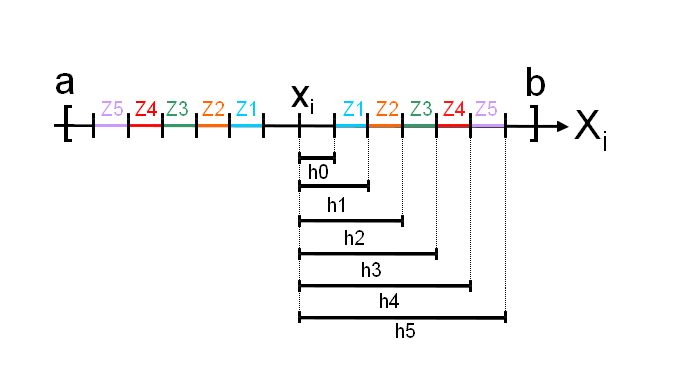
\includegraphics[width=0.7\textwidth,keepaspectratio]{partitionnement_voisinage_CBSO}
	\caption{Partitionnement du voisinage dans CBSO}
\end{figure}


Une zone uni-dimensionnelle $Z_j$ définie par les rayons $h_{j-1}$ et $h_j$ est composée de deux parties égales, une à gauche de $x_i$ et une à droite de $x_i$.

Une variable ($X_j$, $x_j$) est voisine de la variable ($X_i$, $x_i$) si et seulement si elle appartient à une des $k$ zones uni-dimensionnelles. Autrement dit:

$$
|x_i - x_j|\leq h_k
$$

Une variable ($X_j$, $x_j$) n'est pas voisine de la variable ($X_i$, $x_i$) si et seulement si elle n'appartient à aucune des $k$ zones uni-dimensionnelles. Autrement dit:

$$
|x_i - x_j|> h_k
$$ 

\subsubsection{$\bullet\quad$Voisinage d'une solution}
Soit $V$ le symbole dénotant la notion de voisinage. Une solution $s'$ est voisine de la solution $s$ si et seulement si toutes les variables de $s'$ sont voisines de celles de $s$:

$$
s' \in V(s) \Leftrightarrow x'_i \in V(x_i) , \forall i=1,...,n
$$

Une solution $s'$ n'est pas voisine de la solution $s$ si et seulement si toutes les variables de $s'$ ne sont pas voisines de celles de $s$:

$$
s' \notin V(s) \Leftrightarrow x'_i \notin V(x_i) , \forall i=1,...,n
$$

Il est important de s'assurer que les coordonnées de la solution voisine ou non-voisine de $s$ appartiennent au domaine de définition [a,b]. Pour cela, il faut s'assurer que la plus grande zone ne dépasse pas le domaine de définition de la fonction. Autrement dit, le paramètre $h_k$ doit vérifier la contrainte suivante:

$$ 
h_k < \frac{b-a}{2}.
$$

\subsubsection{$\bullet\quad$Détermination d'une solution voisine}

Cela consiste à déterminer les $n$ coordonnées d'une solution $s'$ (une par une) dans la zone définie par les rayons $h_{j-1}$ et $h_j$.

Dans le cas où la valeur $x_i$ de la variable $X_i$ se trouve au milieu du domaine $[a,b]$, il suffit que le générateur de nombres aléatoires choisisse une valeur $x'_i$, telle que:

$$
x'_i\in[x_i-h_{j+1},x_i-h_j] \cup [x_i+h_j,x_i+h_{j+1}]
$$

où:
\begin{itemize}
	\item $x_i$ est la $i^{ème}$ coordonnée de la solution $s$,
	\item $x'_i$ est la $i^{ème}$ coordonnée de la solution voisine.\\
\end{itemize}

Il se peut que la valeur $x_i$ de la variable $X_i$ soit proche de l'une des deux frontières du domaine de définition de la fonction (Figure \ref{debordement}). Dans ce cas, une partie (hachurée) des $k$ zones débordera du domaine [a,b], et seulement l'autre partie (non-hachurée) sera valide et pourra être utilisée pour générer la coordonnée $x'_i$ de la solution non voisine. 

\vspace{-1em}

\begin{figure}[H]
	\centering 
	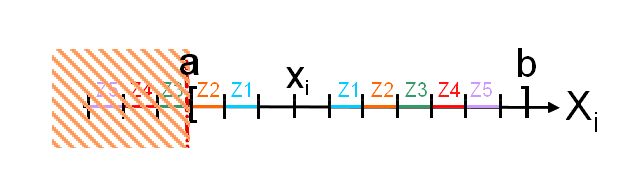
\includegraphics[width=0.7\textwidth,keepaspectratio]{debordement_voisinage2}
	\caption{Débordement du voisinage d'une variable} 
	\label{debordement}
\end{figure}

Si les zones débordent de la borne inférieure, le générateur de nombres aléatoires choisit la valeur $x'_i$ telle que:

$$
x'_i\in[x_i+h_j,x_i+h_{j+1}]
$$

Si les zones débordent de la borne supérieure, le générateur de nombres aléatoires choisit la valeur $x'_i$ telle que:

$$
x'_i\in[x_i-h_{j+1},x_i-h_j]
$$

\subsubsection{$\bullet\quad$Détermination d'une solution non voisine}

Cela consiste à déterminer les coordonnées d'une solution en dehors des $k$ zones.

Dans le cas où la valeur $x_i$ de la variable $X_i$ se trouve au milieu du domaine $[a,b]^2$, il suffit que le générateur de nombres aléatoires choisisse une valeur $x'_i$, telle que:

\begin{equation}
x'_i\in[a,x_i-h_k] \cup [x_i+h_k,b],\label{for1}
\end{equation}

Si les zones débordent de la borne inférieure, alors le générateur de nombres aléatoires choisit la valeur $x'_i$ telle que:

\begin{equation}
x'_i\in[x_i+h_k,b],\label{for2}
\end{equation}

Si les zones débordent de la borne supérieure, le générateur de nombres aléatoires choisit la valeur $x'_i$ telle que:

\begin{equation}
x'_i\in[a,x_i-h_k],\label{for3}
\end{equation}


\parbox[t][]{\textwidth}{}

\vspace{-2.5em}

\subsection{Distance entre deux solutions}
\begin{spacing}{1.6}
Nous avons besoin de cette notion pour le calcul de diversité lors de la phase de diversification. Pour répondre à notre besoin, nous avons choisi la norme $infini$ qui considère le maximum des différences entre les coordonnées des deux solutions. Elle est donnée par la formule:
\end{spacing}

\vspace{0.25em}

$$
Distance(s,s')=\Vert s-s'\Vert_\infty=Max\{\vert x_{1i}-x_{2i} \vert\}, \quad 1\leq i \leq n
$$

\vspace{2em}

où:
\begin{itemize}
	\item $\Vert \cdot \cdot \cdot \Vert_\infty$ est la norme $"infini"$,
	\item $s$ et $s'$ sont deux solutions,
	\item $n$ est la dimension de la fonction problème (le nombre de variables),
	\item $x_{1i}$ est la $i^{ème}$ variable de la première solution,
	\item $x_{2i}$ est la $i^{ème}$ variable de la deuxième solution.\\
\end{itemize}

Par cela, nous définissons notre propre manière de voir la distance entre deux solutions.

\subsection{Diversité d'une solution}

C'est une valeur réelle que nous calculons pour chaque solution de la table $Danse$. Elle est donnée par la formule suivante:

\vspace{-1em}

$$
Diversité(s)= Min\{\Vert s-s' \Vert_\infty , \forall s' \in Tabou\}.
$$


Cette mesure permet d'indiquer à quel point la solution $s$ est éloignée des sommets de référence des itérations précédentes. Rappelons que la liste $Tabou$ contient les anciens sommets de référence.

\vspace{-1em}

\subsection{Algorithme}

\begin{algorithm}[H]
	\caption{CBSO}
	\KwIn{Les paramètres de l'algorithme et la condition d'arrêt}
	\KwOut{La meilleure solution trouvée}
	\Begin{
    Soit $Sref$ la solution trouvée par l'abeille éclaireuse\;
    \While{la condition d'arrêt est non vérifiée}{
      Insérer $Sref$ dans la liste $Tabou$\;
      Déterminer la zone de recherche à partir de $Sref$\;
      Attribuer une solution $s$ de la zone de recherche à chaque abeille\;
      \For{chaque abeille}{
        Recherche locale avec la solution $s$\;
        Mettre l'optimum local dans la table $Danse$\;
      }
      Construire la solution noyau et l'insérer dans la table $Danse$\;
      Choisir le nouveau sommet de référence $Sref$\;
    }
  }
\end{algorithm}

\bigskip

Nous pouvons constater que notre algorithme ne change pas la structure générale de l'algorithme BSO sauf que chaque étape est définie de manière à être mieux adaptée aux problèmes continus.

\subsubsection{$\bullet\quad$Génération du sommet de référence initial}
\begin{spacing}{1.6}
Le sommet de référence initial est construit d'une manière incrémentale (variable par variable). A chaque variable de $Sref$, le générateur de
nombres aléatoires attribue une valeur réelle aléatoire qui obéit à la loi uniforme donnée par la formule suivante:

\begin{equation}
u(x) = \left\{ \begin{array}{rcl}
	\frac{1}{b-a} & \mbox{si}
	& x\in [a,b] \\ 0 & \mbox{sinon}
\end{array}\right.\label{eq2}
\end{equation}


Toutes les valeurs réelles appartenant à l'intervalle $[a,b]$ ont la même probabilité ($p=\frac{1}{b-a}$) d'être choisies et aucune autre valeur ne sera choisie ($p=0$).\\

\subsubsection{$\bullet\quad$Détermination de la zone de recherche}
Elle consiste à générer $m$ solutions à partir du sommet de référence ($m$ étant le nombre d'abeilles) et à attribuer une solution à chaque abeille pour démarrer la recherche locale.

Nous avons considéré quatre abeilles dont les solutions sont distribuées comme suit,

\begin{itemize}
	\item la première abeille travaille sur le sommet de référence. Cela signifie qu'à partir de la deuxième itération, elle va continuer le travail des abeilles de l'itération précédente ($intensifier$ encore plus la recherche),
	\item la deuxième abeille travaille sur une solution non voisine du sommet de référence, pour $diversifier$ la zone de recherche. Cette solution est déterminée en utilisant une des formules \ref{for1}, \ref{for2} ou \ref{for3},
	\item En utilisant le paramètre $Flip$, la troisième abeille combine entre le sommet de référence et une solution non voisine de telle manière à obtenir une \emph{solution hybride}. Nous avons choisi $Flip=2$ ce qui signifie que cette abeille prend les cases impaires du sommet de référence et les cases paires de la solution non voisine.
	
	\vspace{1em}

	\begin{figure}[H]
		\centering
		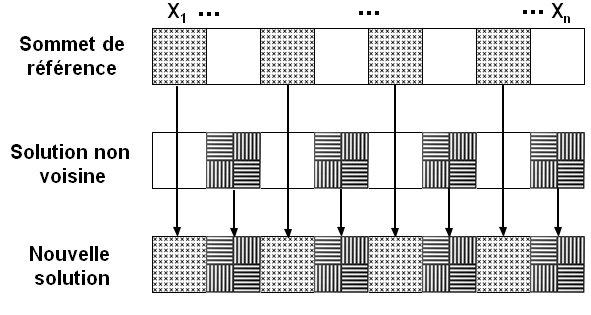
\includegraphics[width=0.8\textwidth,keepaspectratio]{construction_solution}
		\caption{Construction d'une solution à partir de Sref et d'une solution non voisine}
	\end{figure}

	\parbox[][0.5em]{\textwidth}{}

	L'algorithme de construction de la nouvelle solution hybride en utilisant le paramètre $Flip$ est donné comme suit:\\
	
\end{itemize}
	
	\begin{algorithm}[H]
		\KwIn{$Sref$, solution non voisine et $Flip$}
		\KwOut{La nouvelle solution hybride}
		\Begin{
		
				solutionHybride$\leftarrow Sref$\;
				$i\leftarrow Flip$\;
				\While{$i\leq n$}{
					solutionHybride[i]$\leftarrow$ solutionNonVoisine[i]\;
					$i\leftarrow i+Flip$\;
			}
		}
		\caption{Construction de la nouvelle solution}
	\end{algorithm}
\vspace{3em}

\begin{itemize}
	\item la quatrième abeille fait de même que pour la troisième abeille, sauf que la solution obtenue prend les cases paires du sommet de référence et les cases impaires de la solution non voisine.
\end{itemize}
\end{spacing}

\vspace{-0.5em}

\subsubsection{$\bullet\quad$Recherche locale}

\vspace{-0.5em}

Après avoir attribué les solutions de la zone de recherche aux abeilles, chacune d'elles démarre une recherche locale avec sa solution en explorant son voisinage pour éventuellement choisir le voisin qui minimise le plus la fonction objectif.

Après plusieurs expérimentations, nous avons choisi d'opter pour le voisinage en étoile basé sur les deux étapes suivantes:
\begin{itemize}
	\item Générer 5 voisins ($k=5$) tels que les coordonnées de chaque voisin sont prises d'une zone différente ($Z_1,Z_2,...,Z_5$) pour une exploration judicieuse de l'espace de recherche.
	\item Comparer les $k$ voisins générés deux à deux, puis prendre le meilleur et le comparer avec la solution $s$. S'il est meilleur, il sera considéré comme l'optimum local pour cette abeille à cette itération, sinon, la solution $s$ le sera.
\end{itemize}

Le processus de recherche locale est répété un nombre de fois défini par le paramètre $SearchIter$.

\vspace{0.5em}

\begin{algorithm}[H]
	\caption{Recherche locale}
	\KwIn{Solution $s$, $SearchIter$ et $k$}
	\KwOut{Optimum local}
	\Begin{
    \For{$i$ allant de $1$ \KwTo $SearchIter$}{
      \For{$j$ allant de $1$ \KwTo $k$}{
        Générer un voisin $v_i$ dans la $j^{ième}$ zone\;
        \uIf{fitness($v_i$)$ \leftarrow optimum$}
        {
          $\quad\quad$ Retourner $v_i$\;
        }
        \ElseIf{$v_i$ est le meilleur voisin}
        {
          $\quad\quad meilleur\_voisin \leftarrow v_i$\;
        }

      }
      \uIf{fitness($meilleur\_voisin$) $\leq$ fitness($s$)}
      {
        $\quad\quad$Retourner $meilleur\_voisin$\;
      } \Else {Retourner $s$\;}
    }
  }
\end{algorithm}

A la fin de la recherche locale, chaque abeille communique son optimum local à travers la table $Danse$. Celle-ci va donc contenir à la fin de chaque itération, les sommets de référence potentiels de la prochaine itération.

\begin{spacing}{1.4}

\subsubsection{$\bullet\quad$Construction de la solution noyau}

En plus des $m$ optimums locaux existant dans la table $Danse$, nous construisons, à partir de la même table, une autre solution que nous appelons \emph{solution noyau}. Nous nous sommes inspirés de ACO$_\mathbb{R}$ \cite{SOCHA_DORIGO_2006} pour construire cette solution en faisant un choix probabiliste sur ses $n$ composants.

\vspace{1em}

Pour cela, nous utilisons la fonction gaussienne noyau (Gaussian kernel) qui est une distribution de probabilités continue construite à partir de $n$ fonctions gaussiennes individuelles associées aux solutions de la table $Danse$.
\end{spacing}

\parbox[t][1em]{\textwidth}{}

Pour chaque dimension $i$ du problème, il existe une fonction gaussienne noyau $G^i$ différente dont la formule est la suivante:

$$
G^i (x) = \sum^{m}_{j=1} \omega_j \frac{1}{\sigma^i_j \sqrt{2\pi}} \mathrm{e}^{-\frac{(x-\mu^i_j)^2}{2\sigma_j^{i^2}}}
,$$

où:
\begin{itemize}
	\item $m$ est le nombre de solutions dans la table $Danse$,
	\item $\omega_j$ est le poids associé à la $j^{ème}$ solution donné par son rang (la solution qui a la meilleure évaluation aura le plus grand poids et celle qui a la pire évaluation aura le plus petit poids),
	\item $\mu^i$ est le vecteur des moyennes,
	\item $\sigma^i$ est le vecteur des écart-types.\\
\end{itemize} 

\begin{figure}[H]
	\centering
	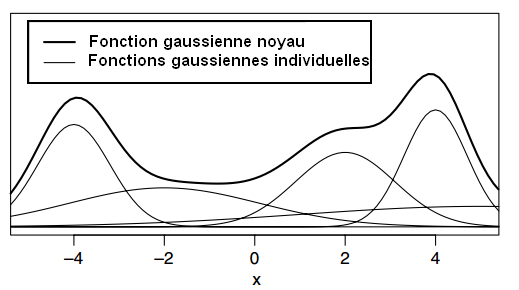
\includegraphics[width=0.8\textwidth,keepaspectratio]{representation_gauss}
	\caption[Représentation graphique de la fonction gaussienne noyau]{Représentation graphique de la fonction gaussienne noyau \cite{SOCHA_DORIGO_2006}}
\end{figure}

La fonction gaussienne noyau nous permet de détecter les régions prometteuses à partir des optimums locaux trouvés par les abeilles. Cela nous aide à nous rapprocher encore de l'optimum global.

Le processus de construction de la nouvelle solution est appelé échantillonnage de la fonction gaussienne noyau et est défini pratiquement, pour chaque dimension $i$ du problème, par:

\begin{itemize}
	\item le choix de la meilleure solution $s_l$ dans la table $Danse$,
	\item le calcul des valeurs $\mu^i_l$ et $\sigma^i_l$ associées à $s_l$,
	\item l'appel au générateur de nombre aléatoires gaussien qui prend en entrée $\mu^i_l$ et $\sigma^i_l$ et retourne une valeur réelle aléatoire $x$ qui obéit à la loi gaussienne $N(\mu^i_l,\sigma^i_l)$ donnée par la formule:
	$$
	g(x)= \frac{1}{\sigma^i_l \sqrt{2\pi}} \mathrm{e}^{-\frac{(x-\mu^i_l)^2}{2\sigma_l^{i^2}}} \quad ,\quad x \in [a,b].
	$$
	 .
\end{itemize} 

$\mu^i_l$ est tout simplement la $i^{ème}$ valeur de la meilleure solution ($\mu^i_l=s^i_l$).

L'écart-type $\sigma^i_l$ représente une erreur moyenne entre la $i^{ème}$ valeur de $s_l$ et celles des autres solutions et se calcule par la formule suivante:

$$
\sigma_l^i = \xi \sum_{j=1}^{m} \frac{|S_j^i - S_l^i|}{m-1}.
$$

où $\xi$ est le paramètre qui contrôle la vitesse de convergence de la solution noyau.

Après la construction de la solution noyau, nous l'évaluons et l'insérons dans la table $Danse$, puis nous choisissons le prochain sommet de référence.

\subsubsection{$\bullet\quad$Choix du nouveau sommet de référence}
Lorsqu'il s'agit des fonctions multi-modales (à plusieurs optimums locaux), il est très important que l'algorithme évite d'être stagné dans un optimum local. Pour cela, il faut utiliser une stratégie de diversification de recherche afin de pouvoir converger vers l'optimum global. 

En réalité, ce sont deux buts contradictoires. D'une part, un algorithme est supposé converger le plus vite possible et d'autre part, il est supposé ne pas converger entièrement vers un optimum local.

Cette contradiction est due au fait q'un algorithme ne peut pas savoir si une région prometteuse mène à un optimum local ou à un optimum global. Le défi est d'établir une balance entre l'efficacité (diversification) et la rapidité (intensification). Cela se traduit par la capacité de choisir le bon prochain sommet de référence à partir de la table $Danse$ qui contient $m+1$ solutions.

Soient:

\begin{itemize}
	\item $Sref_t$ le sommet de référence à l'instant $t$,
	\item $Sref_{t+1}$ le sommet de référence à l'instant $t+1$,
	\item $MSolutionQualité$ la meilleure solution en qualité à l'instant $t$,
	\item $MSolution Diversité$ la meilleure solution en diversité à l'instant $t$.
\end{itemize}

\begin{algorithm}[H]
	\caption{Choix du nouveau sommet de référence}
	\KwIn{La table $Danse$}
	\KwOut{Le nouveau sommet de référence $Sref_{t+1}$}
	\Begin{
		\uIf{fitness($MSolutionQualité$) $\leq$ fitness($Sref_t$)\tcc{La meilleure solution à cette itération est meilleure que $Sref_t$} }
				{
					$\quad\quad Sref_{t+1} \leftarrow MSolutionQualité$\;
					
					$\quad\quad NbChances \leftarrow MaxChances$\;
				}
				\Else
				{
					$\quad\quad$ \tcc{La meilleure solution à cette itération est pire que $Sref_t$}
					
					$\quad\quad NbChances \leftarrow NbChances-1$\;
					
					\uIf{$NbChances > 0$ }
					{
						$\quad\quad Sref_{t+1} \leftarrow MSolutionQualité$\;
					}
				
					\Else
					{	
					$\quad\quad Sref_{t+1} \leftarrow MSolutionDiversité$\;
					
					$\quad\quad NbChances \leftarrow MaxChances$\;	
					}		
				}	
	}
\end{algorithm}
\bigskip

Si la meilleure solution en qualité (celle qui a la plus petite évaluation) est meilleure que le sommet de référence, elle sera considérée comme le prochain sommet de référence. Sinon, elle le sera quand même sauf que nous décrémentons le nombre de chances. Si le nombre de chances devient nul, la meilleure solution en diversité (celle qui a la plus grande diversité) sera considérée comme le prochain sommet de référence et le nombre de chances sera réinitialisé à son maximum.

\begin{itemize}
	\item Lors du choix de la meilleure solution en qualité (instructions $4$ et $10$), si deux solutions ont la même qualité, celle qui a la plus grande diversité sera considérée.
	\item Lors du choix de la meilleure solution en diversité (instruction $12$), si deux solutions ont la même diversité, celle qui a la plus petite évaluation (meilleure qualité) sera considérée. 
\end{itemize} 
 
Il est important que la meilleure solution (en qualité ou en diversité) choisie ne soit pas taboue. Si elle l'est, nous choisissons la prochaine meilleure solution et ainsi de suite. Il peut arriver, même rarement, que toutes les solutions de la table $Danse$ soient taboues. Dans ce cas, le prochain sommet de référence sera généré aléatoirement selon la loi uniforme (équation \ref{eq2}).

\subsubsection{$\bullet\quad$Condition d'arrêt}
Les instructions $5$ à $12$ de l'algorithme CBSO sont répétées jusqu'à ce qu'une de ces trois conditions soient vérifiées: 

\begin{itemize}
	\item l'algorithme converge vers la solution souhaitée ($\vert f-f^* \vert < \epsilon$ où $\epsilon$ est un paramètre de l'algorithme),
	\item le nombre maximum des itérations est atteint, 
	\item une stagnation est détectée (on n'aperçoit pas de changement dans le sommet de référence au bout d'un nombre d'itérations défini par le paramètre $Stag$). 
\end{itemize} 
 
\section*{Conclusion}
Nous avons présenté dans ce chapitre l'adaptation de la méta-heuristique BSO aux problèmes d'optimisation continue. Nous passons à présent à l'implémentation de notre algorithme.

	\chapter {Implémentation de l'algorithme}
\section*{Introduction}
Dans ce chapitre, nous expliquons l'environnement de travail que nous avons utilisé afin d'implémenter CBSO, puis nous présentons l'interface graphique de notre application.\\

\section{Outils de travail}
Nous avons eu besoin des outils suivants:

\begin{itemize}
	\item langage de programmation Java,
	\item environnement de développement Netbeans,
	\item machine dotée d'un processeur Intel core i3 et d'une RAM de 4GO. 
\end{itemize}

\bigskip

\section{Application}
L'interface graphique de notre application aide l'utilisateur à paramétrer l'algorithme et à l'exécuter sur les différentes fonctions de test.

Les paramètres de l'algorithme sont chargés automatiquement à l'apparition de l'interface graphique, ils peuvent être changés par l'utilisateur.\\\\
\bigskip\bigskip\bigskip
\vspace{6em}

Les figures suivantes montrent l'interface graphique avec les différentes étapes d'utilisation.

\begin{figure}[H]
	\centering
	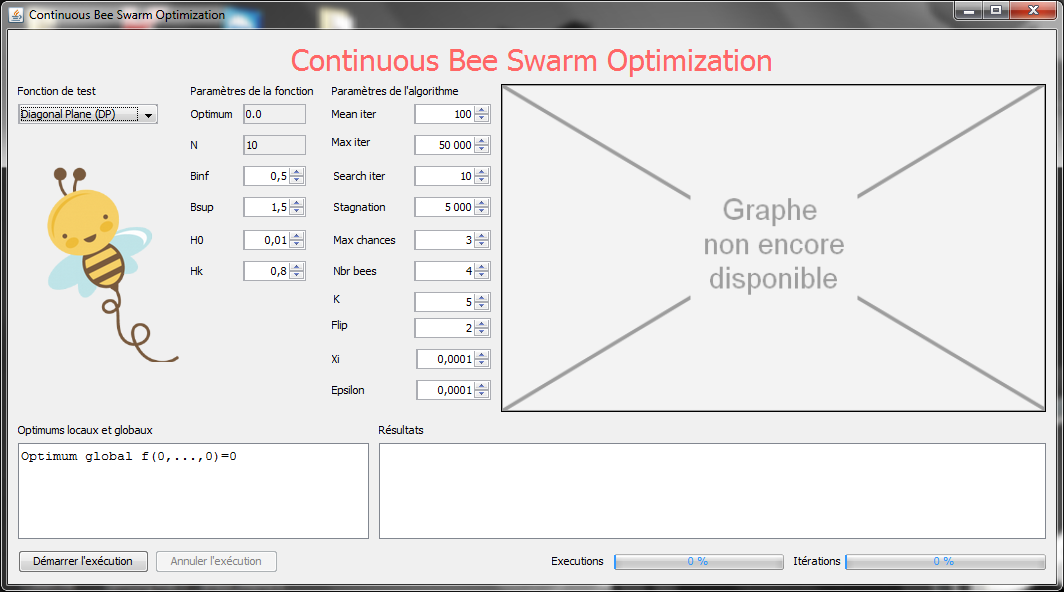
\includegraphics[width=\textwidth,keepaspectratio]{IHM1}
	\caption{Interface graphique de l'application}
\end{figure}

\bigskip \bigskip 
Il suffit que l'utilisateur passe le curseur sur le nom d'un paramètre pour qu'une information explicative de ce dernier apparaisse.\\\\


\begin{figure}[H]
	\centering
	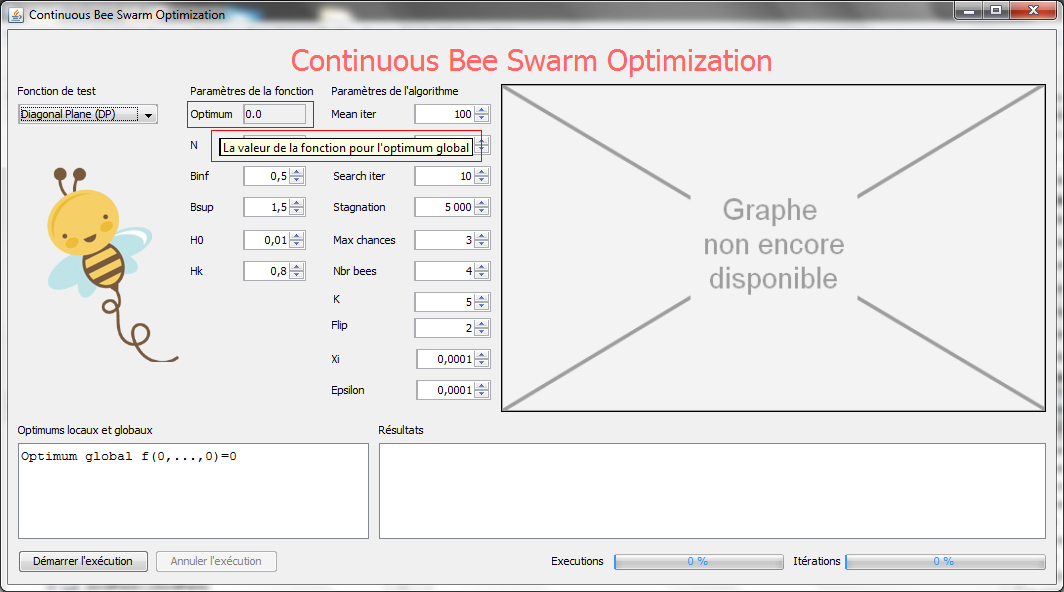
\includegraphics[width=\textwidth,keepaspectratio]{IHM2}
	\caption{Explication des paramètres de l'algorithme}
\end{figure}

\bigskip \bigskip \bigskip 

L'utilisateur commence  par choisir la fonction de test à partir de la liste déroulante qui se trouve en haut à gauche de l'interface.

\begin{figure}[H]
	\centering
	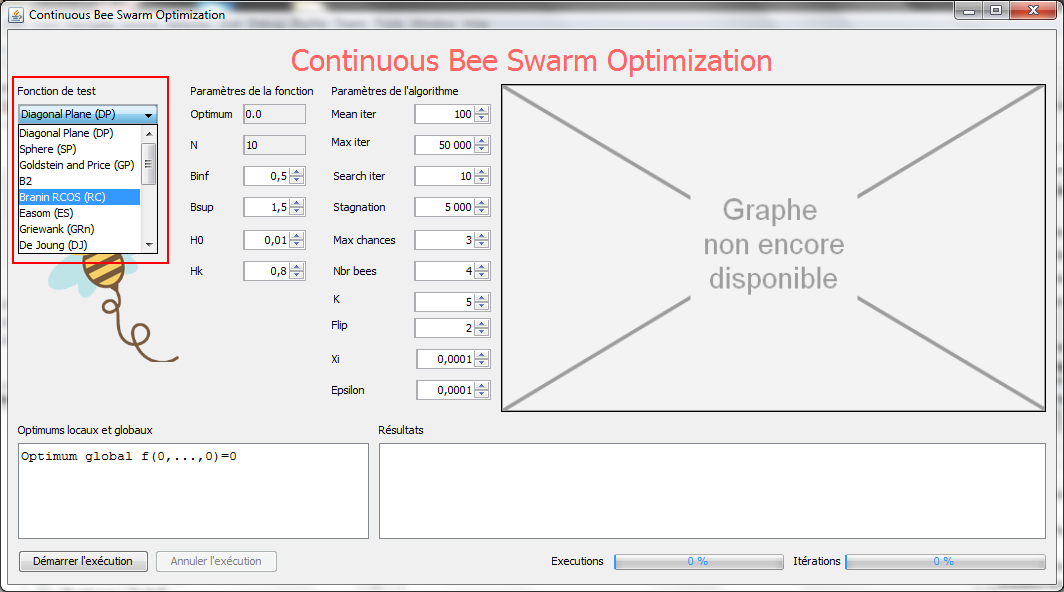
\includegraphics[width=\textwidth,keepaspectratio]{IHM3}
	\caption{Choix de la fonction de test}
\end{figure}
\vspace{-2em}
Après avoir choisi la fonction, ses paramètres sont chargés automatiquement. L'utilisateur peut choisir de travailler sur un sous-domaine du domaine de définition de la fonction comme il peut changer les paramètres $h_0$ et $h_k$.

\begin{figure}[H]
	\centering
	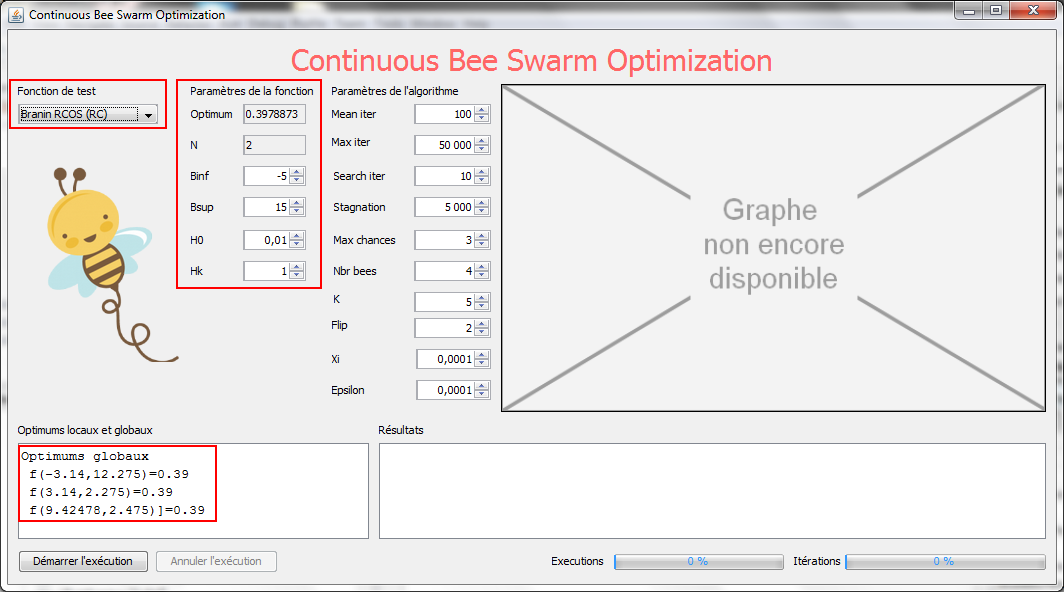
\includegraphics[width=\textwidth,keepaspectratio]{IHM4}
	\caption{Chargement des paramètres de la fonction de test}
\end{figure}
\vspace{-2em}
Avant de lancer CBSO, l'utilisateur peut fixer le nombre d'exécutions indépendantes de l'algorithme à travers le paramètre $MeanIter$. Nous avons fixé par défaut ce nombre à $100$ itérations indépendantes et cela pour avoir des résultats plus fiables.

L'utilisateur peut alors lancer CBSO en appuyant sur le bouton \emph{Démarrer l'exécution}. La progression de l'algorithme est observée à travers deux barres de progression, la première indiquant le numéro de l'exécution courante et la deuxième le numéro d'itération courante dans l'exécution.


\begin{figure}[H]
	\centering
	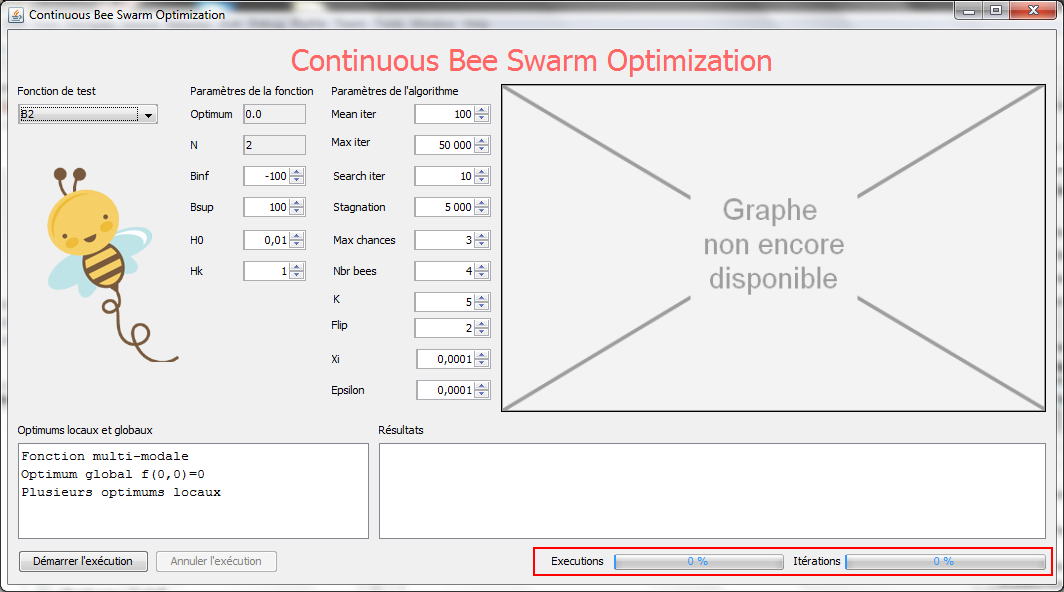
\includegraphics[width=\textwidth,keepaspectratio]{IHM5}
	\caption{Barres de progression}
\end{figure}

Dans le cas où l'utilisateur veut interrompre l'exécution, il appuie sur le bouton \emph{Annuler l'exécution}.
\begin{figure}[H]
	\centering
	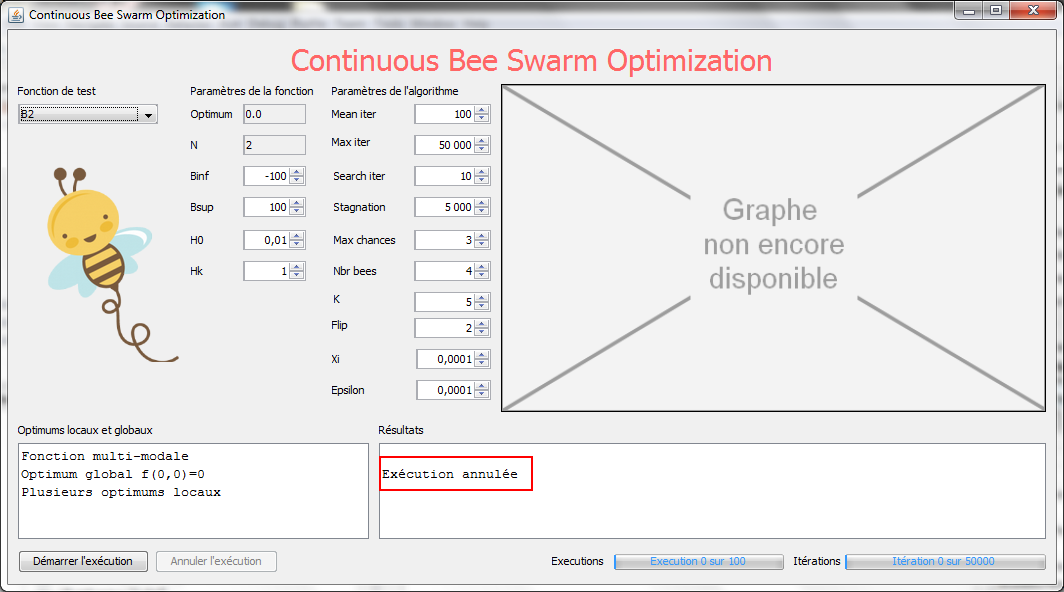
\includegraphics[width=\textwidth,keepaspectratio]{IHM6}
	\caption{Annulation de l'exécution}
\end{figure}

A la fin de l'algorithme, les informations concernant l'exécution sont affichées dans la zone de texte en bas à droite. Ces informations comportent la meilleure solution trouvée, le nombre des itérations, le nombre des évaluations de la fonction, le taux de réussite, de stagnation et d'atteinte de $MaxIter$ ainsi que le temps d'exécution.

\vspace{0.5em}

De plus, un graphe est affiché représentant l'évolution de l'évaluation du sommet de référence à travers les 3000 premières itérations au maximum de la dernière exécution.

\begin{figure}[H]
	\centering
	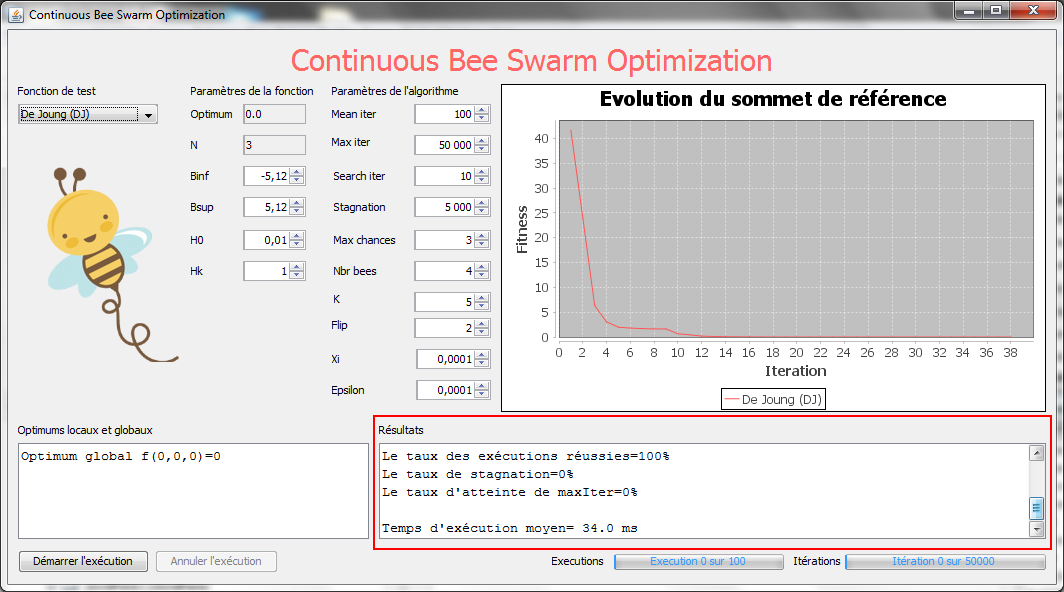
\includegraphics[width=\textwidth,keepaspectratio]{IHM7}
	\caption{Affichage des résultats}
\end{figure}

\section*{Conclusion}
Après avoir présenté l'interface graphique de l'application, l'étape suivante est celle du test et de l'évaluation de CBSO.

	\chapter{Expérimentations et résultats}

\section*{Introduction}
En général, il y a deux catégories de problèmes d'optimisation, les fonctions de test et les problèmes du monde réel. Les fonctions de test sont des problèmes artificiels qui peuvent être utilisés pour l'évaluation d'un algorithme dans différentes situations avec plusieurs niveaux de difficulté.

Les problèmes du monde réel touchent à différents domaines tels la physique, la chimie, l'ingénierie et les mathématiques. Ces problèmes sont plus difficiles à manipuler que les fonctions de test artificielles, mais ils se ramèment toujours à une ou à plusieurs d'entre elles.

Après l'implémentation de CBSO, nous pouvons donner les fonctions de test utilisées ainsi que les paramètres de l'algorithme. Ensuite, nous présentons les résultats de nos expérimentations qui sont une phase très importante pour l'évaluation de notre travail. Enfin, nous faisons une étude comparative entre CBSO et d'autres algorithmes d'optimisation continue en vue d'examiner les performances de CBSO et sa capacité de converger vers l'optimum global face aux fonctions multimodales.

\section{Fonctions de test}
Nous avons mené nos expérimentations sur des benchmarks publics utilisés par des méthodes avec lesquelles nous envisageons une comparaison. Ces benchmarks contiennent des fonctions de test de plusieurs types dont les optimums globaux sont connus.

Les fonctions multi-modales avec plusieurs optimums locaux sont parmi les classes de problèmes les plus difficiles, tandis que les fonctions à surfaces plates posent une difficulté à l'algorithme parce qu'elles ne donnent pas d'information pour le diriger vers l'optimum. 

\vspace{2em}La liste des fonctions de test que nous avons utilisées est la suivante\cite{Momin_Yang_2013}.
\begin{itemize}
	\item
	Diagonal Plane ($DP$)\\$$DP(\overrightarrow{x})=\frac{1}{n}\sum_{i=1}^{n} x_i$$
	
	\begin{itemize}[label={$\circ$}]
		\item $n=$10, 
		\item $\overrightarrow{x} \in [0.5,1.5]^n$,
		\item $h_0=10^{-22}$,
		\item $h_k=7*10^{-21}$,
		\item optimum global DP(0.5,...,0.5)=0.5,
		\item continue, non-séparable et uni-modale.
	\end{itemize}
	
	\bigskip
	\bigskip
	\item
	Sphere ($SP$)\\$$SP(\overrightarrow{x})=\sum_{i=1}^{n} x_i^2$$

	\begin{itemize}[label={$\circ$}]  
		\item $n=$10, 
		\item $\overrightarrow{x} \in [-3,7]^n$,
		\item $h_0=10^{-5}$,
		\item $h_k=10^{-1}$,
		\item optimum global SP(0,...,0)=0,
		\item continue, séparable et multi-modale.
	\end{itemize}
	
	\bigskip
	\bigskip
	\item
	$B_2$\\$$B_2(\overrightarrow{x})=(x_1^2+2x_2^2-0.3\cos(3\pi x_1)-0.4\cos(4\pi x_2)+0.7)$$

	\begin{itemize}[label={$\circ$}]
		\item $n=$2,
		\item $\overrightarrow{x} \in [-100,100]^n$,
		\item $h_0=3*10^{-3}$,
		\item $h_k=2$,
		\item optimum global B$_2$(0,0)=0,
		\item continue, non-séparable et multi-modale.
	\end{itemize}
	
	\bigskip
	\bigskip
	\item
	Branin RCOS 
	($RC$)\\$$RC(\overrightarrow{x})=\left(x_2-\left(\frac{5}{(4\pi^2)}\right)x_1^2+\left(\frac{5}{\pi}\right)x_1-6\right)^2+10\left(1-\left(\frac{1}{8\pi}\right)\right)\cos(x_1) +10$$

	\bigskip

	\begin{itemize}[label={$\circ$}]
		\item $n=$2, 
		\item $\overrightarrow{x} \in [-5,15]^n$,
		\item $h_0=6*10^{-4}$,
		\item $h_k=8*10^{-1}$,
		\item optimums globaux RC(-$\pi$,12.275)=0.39, RC($\pi$,2.275)=0.39, RC(9.42478,2.475)=0.39,
		\item continue, non-séparable et multi-modale.
	\end{itemize}
	
	\bigskip
	\bigskip
	\item
	Easom ($ES$)\\$$ES(\overrightarrow{x})= -\cos (x_1)\cos (x_2) \exp (-((x_1-\pi )^2+(x_2-\pi)^2))$$

	\begin{itemize}[label={$\circ$}]
		\item $n=$2,
		\item $\overrightarrow{x} \in [-100,100]^n$,
		\item $h_0=8*10^{-4}$,
		\item $h_k=2$,
		\item optimum global ES($\pi$,$\pi$)=-1,
		\item continue, séparable et multi-modale.
	\end{itemize}
	
	\bigskip
	\bigskip
	\item
	De Joung ($DJ$)\\$$DJ(\overrightarrow{x})= x_1^2+x_2^2+x_3^2$$
	
	\begin{itemize}[label={$\circ$}]
		\item $n=$3, 
		\item $\overrightarrow{x} \in [-5.12,5.12]^n$,
		\item $h_0=3*10^{-4}$,
		\item $h_k=4*10^{-1}$,
		\item optimum global DJ(0,0,0)=0,
		\item continue, séparable et multi-modale.
	\end{itemize}
	
	\bigskip
	\bigskip
		\bigskip
	\bigskip
	\item
	Rosenbrock2 ($R_2$)\\$$R_n(\overrightarrow{x})= \sum_{i=1}^{n-1} [100(x_i^2-x_{i+1})^2+(x_i -1)^2]$$
	\begin{itemize}[label={$\circ$}]
		\item $n=$2, 
		\item $\overrightarrow{x} \in [-5,10]^n$,
		\item $h_0=10^{-2}$,
		\item $h_k=1$,
		\item optimum global R$_n$(1,...,1)=0,
		\item continue, non-séparable et uni-modale.
	\end{itemize}
	\bigskip
	\item Zakharov2 ($Z_2$)
	
	\bigskip
	
	$$Z_n(\overrightarrow{x})= \left(\sum_{i=1}^{n}x_i^2\right) + \left(\sum_{i=1}^{n} 0.5ix_i\right)^2 + \left(\sum_{i=1}^{n} 0.5ix_i\right)^4$$
	
	\bigskip
	
	\begin{itemize}[label={$\circ$}]
		\item $n=$2,
		\item $\overrightarrow{x} \in [-5,10]^n$,
		\item $h_0=10^{-2}$,
		\item $h_k=2*10^{-1}$,
		\item optimum global Z$_n$(0,...,0)=0,
		\item continue, non-séparable et multi-modale.
	\end{itemize}
	
	\bigskip
	\bigskip
	\item Zakharov5 ($Z_5$)\\$$Z_n(\overrightarrow{x})= \left(\sum_{i=1}^{n}x_i^2\right) + \left(\sum_{i=1}^{n} 0.5ix_i\right)^2 + \left(\sum_{i=1}^{n} 0.5ix_i\right)^4$$
	
	\begin{itemize}[label={$\circ$}]
		\item $n=$5,
		\item $\overrightarrow{x} \in [-5,10]^n$,
		\item $h_0=2*10^{-3}$,
		\item $h_k=2*10^{-1}$,
		\item optimum global Z$_n$(0,...,0)=0,
		\item continue, non-séparable et multi-modale.
	\end{itemize}
	\bigskip
	\bigskip
	\item
	Hartmann$_3$ ($H_{3,4}$)\\$$H_{3,4}(\overrightarrow{x})= -\sum_{i=1}^{4} c_i \exp[-\sum_{j=1}^{3}a_{ij}(x_j-p_{ij})^2]$$
	
	\begin{itemize}[label={$\circ$}]
		\item $n=$3, 
		\item $\overrightarrow{x} \in [0,1]^n$,
		\item $h_0=6*10^{-5}$,
		\item $h_k=8*10^{-2}$,
		\item optimum global H$_{3,4}$(0.1140,0.556,0.852)=-3.86,
		\item continue, non-séparable et multi-modale (4 optimums locaux).
	\end{itemize}
	
	\bigskip
	
	\begin{table}[H]\centering
		\begin{tabular}{ccc|c|ccc}
			\toprule \textbf{} & \textbf{$a_{ij}$} & \textbf{} & \textbf{$c_i$} & \textbf{} & \textbf{$p_{ij}$}  \\    \midrule
			3.0 & 10. & 30. & 1.0 &0.3689 &0.1170 &0.2673   \\  
			0.1 & 10. & 35. & 1.2 &0.4699 &0.4387 &0.7470   \\ 
			3.0 & 10. & 30. & 3.0 &0.1091 &0.8732 &0.5547   \\
			0.1 & 10. & 35. & 3.2 &0.0381 &0.5743 &0.8828   \\ 
			\bottomrule	
		\end{tabular}
	\end{table}
	\bigskip
	\bigskip
	\item
	Hartmann$_6$ ($H_{6,4}$)\\$$H_{6,4}(\overrightarrow{x})= -\sum_{i=1}^{4} c_i \exp[-\sum_{j=1}^{6}a_{ij}(x_j-p_{ij})^2]$$

	\begin{itemize}[label={$\circ$}]
		\item $n=$6, 
		\item $\overrightarrow{x} \in [0,1]^n$,
		\item $h_0=10^{-3}$,
		\item $h_k=2*10^{-2}$,
		\item optimum global H$_{6,4}$(0.2016,0.1500,0.4768,0.2753,0.3116,0.6573)=-3.32,
		\item continue, non-séparable et multi-modale (4 optimums locaux).
	\end{itemize}

	\bigskip

	\begin{table}[H]\centering
		\begin{tabular}{cccccc|c|cccccc}
			\toprule \textbf{} & \textbf{} & \textbf{$a_{ij}$} & \textbf{} & \textbf{} & \textbf{} & \textbf{$c_i$} & \textbf{} & \textbf{} & \textbf{} & \textbf{$p_{ij}$} & \textbf{} & \textbf{}  \\    \midrule
			10. & 3. & 17. & 3.5 & 1.7 & 8. & 1.0 & 0.1312 & 0.1696 & 0.5569 & 0.0124 & 0.8283 & 0.5886 \\  
			0.05 & 10. & 17. & 0.1 & 8.0 & 14.0 & 1.2 & 0.2329 & 0.4135 & 0.8307 &0.3736 & 0.1004 & 0.9991  \\ 
			3.0 & 3.5 & 1.7 & 10.0 & 17.0 & 8.0 & 3.0 & 0.2348 & 0.1451 & 0.3522 & 0.2883 & 0.3047 & 0.6650  \\
			17.0 & 8.0 & 0.05 & 10.0 & 0.1 & 14.0 & 3.2 & 0.4047 & 0.8828 & 0.8732 & 0.5743 &0.1091 &0.0381  \\ 
			\bottomrule	
		\end{tabular}
	\end{table}
	\vspace{5em}
	\item Shekel$_5$ ($S_{4,5}$)\\$$S_{4,5}(\overrightarrow{x})= -\sum_{i=1}^{5} [(\overrightarrow{x}-a_i)^T(\overrightarrow{x}-a_i)+c_i]^{-1}$$

	\begin{itemize}[label={$\circ$}]
		\item $n=$4, 
		\item $\overrightarrow{x} \in [0,10]^n$,
		\item $h_0=6*10^{-5}$,
		\item $h_k=2*10^{-2}$,
		\item optimum global S$_{4,5}$(4,4,4,4)=-10.14,
		\item continue, non-séparable et multi-modale (5 optimums locaux).
	\end{itemize}

	\bigskip

	\begin{table}[H]\centering
		\begin{tabular}{cccc|c}
			\toprule \textbf{} & \textbf{$a_{ij}$} & \textbf{} & \textbf{} & \textbf{$c_i$}\\    \midrule
			4 & 4 & 4 & 4 & 0.1    \\  
			1 & 1 & 1 & 1 & 0.2   \\ 
			8 & 8 & 8 & 8 & 0.2  \\
			6 & 6 & 6 & 6 & 0.4   \\ 
			3 & 7 & 3 & 7 & 0.4 \\ 
			\bottomrule	
		\end{tabular}
	\end{table}

	\bigskip

	\item Shekel$_7$ ($S_{4,7}$)\\$$S_{4,7}(\overrightarrow{x})= -\sum_{i=1}^{7} [(\overrightarrow{x}-a_i)^T(\overrightarrow{x}-a_i)+c_i]^{-1}$$

	\begin{itemize}[label={$\circ$}]
		\item $n=$4, 
		\item $\overrightarrow{x} \in [0,10]^n$,
		\item $h_0=6*10^{-5}$,
		\item $h_k=2*10^{-2}$,
		\item optimum global S$_{4,7}$(4,4,4,4)=-10.39,
		\item continue, non-séparable et multi-modale (7 optimums locaux).
	\end{itemize}

	\bigskip

	\begin{table}[H]\centering
		\begin{tabular}{cccc|c}
			\toprule \textbf{} & \textbf{$a_{ij}$} & \textbf{} & \textbf{} & \textbf{$c_i$} \\    \midrule
			4 & 4 & 4 & 4 & 0.1    \\  
			1 & 1 & 1 & 1 & 0.2   \\ 
			8 & 8 & 8 & 8 & 0.2  \\
			6 & 6 & 6 & 6 & 0.4   \\ 
			3 & 7 & 3 & 7 & 0.4 \\ 
			2 & 9 & 2 & 9 & 0.6   \\ 
			5 & 5 & 3 & 3 & 0.3 \\ 
			\bottomrule	
		\end{tabular}
	\end{table}
	
	\bigskip
	\bigskip
	\bigskip
	\item Shekel$_{10}$ ($S_{4,10}$)
	
	\bigskip
	$$S_{4,10}(\overrightarrow{x})= -\sum_{i=1}^{10} [(\overrightarrow{x}-a_i)^T(\overrightarrow{x}-a_i)+c_i]^{-1}$$
	\begin{itemize}[label={$\circ$}]
		\item $n=$4, 
		\item $\overrightarrow{x} \in [0,10]^n$,
		\item $h_0=6*10^{-5}$,
		\item $h_k=2*10^{-2}$,
		\item optimum global S$_{4,10}$(4,4,4,4)=-10.53,
		\item continue, non-séparable et multi-modale (10 optimums locaux).
	\end{itemize}

	\bigskip
	\bigskip
	
	\begin{table}[H]\centering
		\begin{tabular}{cccc|c}
			\toprule \textbf{} & \textbf{$a_{ij}$} & \textbf{} & \textbf{} & \textbf{$c_i$} \\    \midrule
			4 & 4 & 4 & 4 & 0.1  \\  
			1 & 1 & 1 & 1 & 0.2  \\ 
			8 & 8 & 8 & 8 & 0.2  \\
			6 & 6 & 6 & 6 & 0.4  \\ 
			3 & 7 & 3 & 7 & 0.4  \\ 
			2 & 9 & 2 & 9 & 0.6  \\ 
			5 & 5 & 3 & 3 & 0.3  \\ 
			8 & 1 & 8 & 1 & 0.7  \\ 
			6 & 2 & 6 & 2 & 0.5  \\ 
			7 & 3.6 & 7 & 3.6 & 0.5  \\ 
			\bottomrule	
		\end{tabular}
	\end{table}
	
\end{itemize}

\vspace{1.5em}

Comme nous l'avons expliqué, la représentation graphique d'une fonction est impossible si elle comporte plus de deux variables. Nous donnons ici la représentation de quelques fonctions à deux variables :

\begin{figure}[H]
	\centering
	\begin{subfigure}{0.3\textwidth}
		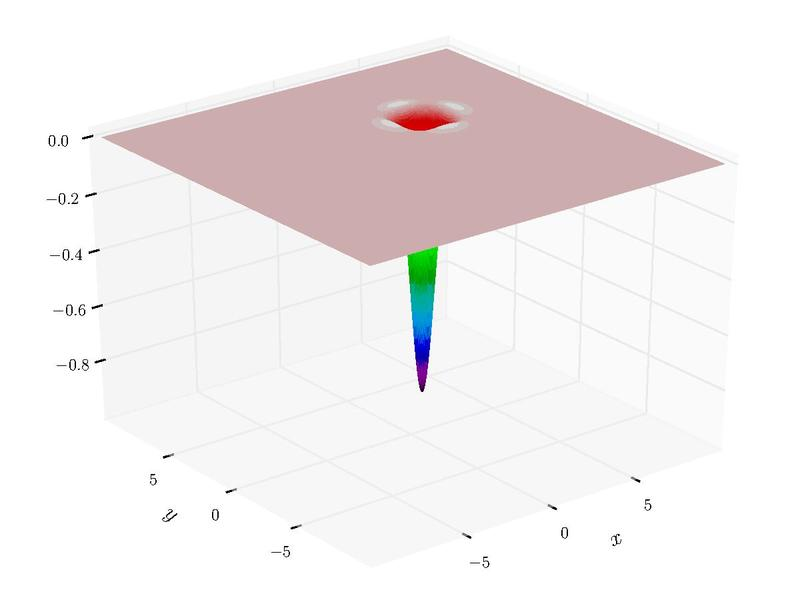
\includegraphics[width=\textwidth]{ES}
		\caption{Easom}
	\end{subfigure}
	\begin{subfigure}{0.3\textwidth}
		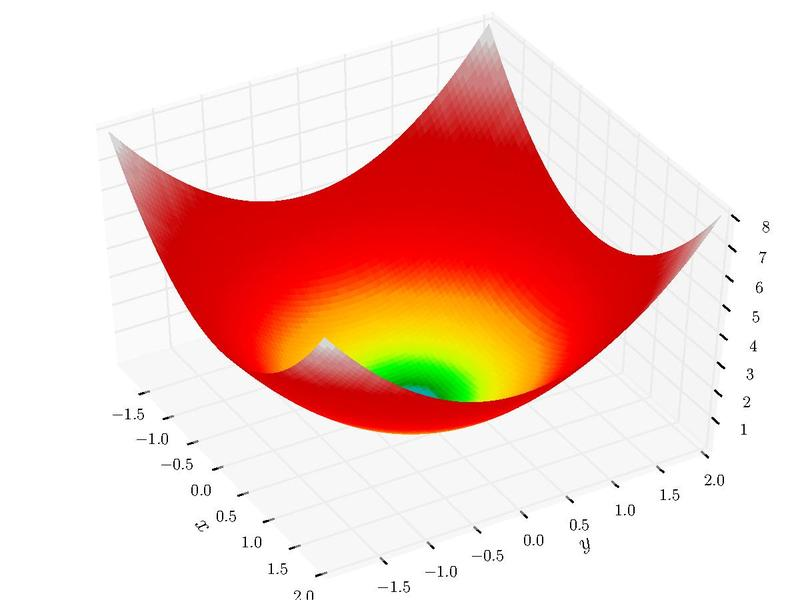
\includegraphics[width=\textwidth]{SP}
		\caption{Sphere}
	\end{subfigure}
	\begin{subfigure}{0.3\textwidth}
		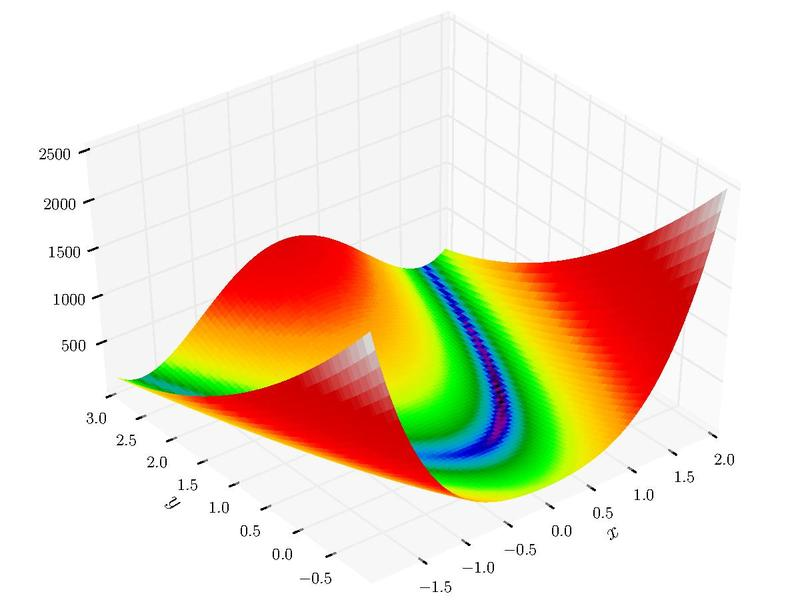
\includegraphics[width=\textwidth]{R}
		\caption{RosenBrock2}
	\end{subfigure}
	\caption{Représentation graphique de quelques fonctions de test à deux variables}
\end{figure}

\section{Paramètres de CBSO}
Chaque algorithme d'optimisation est caractérisé par un certain nombre de paramètres qui le définissent et le guident dans le processus de recherche de solution. La liste des paramètres que nous avons utilisés dans CBSO est la suivante.

\begin{table}[H]\centering
	\begin{tabular}{cp{0.5\textwidth}c}
		\toprule \textbf{Paramètre} & \textbf{Signification} & \textbf{Valeur}  \\    \midrule
		$m$ & Nombre d'abeilles. & $4$   \\   
		$k$ & Nombre de voisins. & $5$  \\   
		$SearchIter$ & Nombre d'itérations d'une recherche locale. & $10$ \\   
		$\xi$ & Vitesse de convergence de la solution noyau. & $0.0001$  \\     \addlinespace 
		$Stag$ & Nombre toléré d'itérations avant de détecter la stagnation. & $5000$ \\ \addlinespace 
		$MaxChances$ & Nombre maximum de chances pour améliorer le sommet de référence. & $3$   \\ \addlinespace 
		$1/Flip$ & Pourcentage de variables à remplacer dans le $SRef$. & 1/2   \\ \addlinespace 
		$MaxIter$ & Nombre maximum des itérations pour trouver la solution. & $50000$  \\ \addlinespace 
		$\epsilon$ & Précision voulue: différence tolérée entre l'évaluation de la solution et l'optimum global. & $10^{-4}$   \\		
		\bottomrule	
	\end{tabular}
	\caption{Paramètres de CBSO\label{key}}
\end{table}

\vspace{-1.2em}

\section{Analyse de CBSO}

\vspace{-0.5em}

Comme nous l'avons précisé, l'utilisateur visualise, à partir de l'interface graphique, le graphe représentant l'évolution de l'évaluation du sommet de référence au cours des itérations. La figure suivante montre ce graphe pour la fonction \emph{De Joung}.\bigskip

\begin{figure}[H]
	\centering
	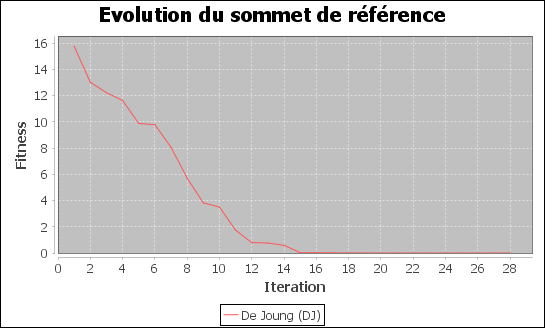
\includegraphics[width=0.65\textwidth,keepaspectratio]{DeJoung}
	\caption{Evolution de $SRef$ pour la fonction $De~Joung$}
\end{figure}

Nous remarquons que CBSO converge bien vers l'optimum. En commençant à partir d'une solution aléatoire qui a une grande évaluation, l'algorithme se rapproche petit à petit de la solution qui a la plus petite évaluation.

Lorsqu'il s'agit des fonctions multi-modales, nous remarquons des sauts dans l'évaluation du sommet de référence dans le graphe. Ces pics indiquent les moments de diversification où l'algorithme décide à régresser pour mieux avancer. Cela se traduit par un changement de la région à explorer de l'espace de recherche.

Nous donnons comme exemple la fonction multi-modale $Shekel_{4,10}$.\bigskip
\begin{figure}[H]
	\centering
	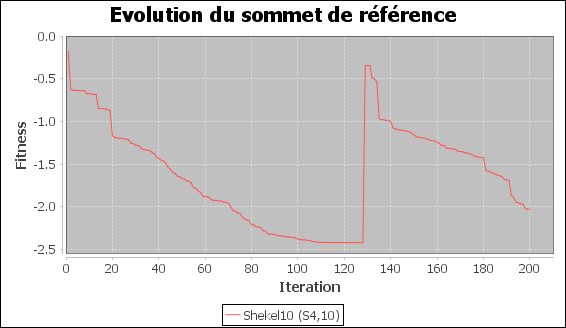
\includegraphics[width=0.65\textwidth,keepaspectratio]{Shekel}
	\caption{Evolution de $SRef$ pour la fonction $Shekel_{4,10}$}
\end{figure}

Pour simplifier, supposons que nous sommes face à une fonction à une seule variable. La figure suivante montre l'utilité de diversification en cas de stagnation dans un optimum local.

\begin{figure}[H]
	\centering
	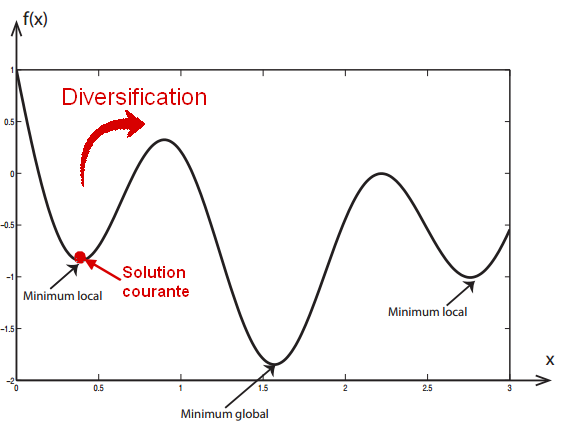
\includegraphics[width=0.70\textwidth,keepaspectratio]{diversification}
	\caption{Utilité de la diversification pour le changement de la zone de recherche}
\end{figure}

La diversification dans CBSO est faite lorsque le nombre de chances pour améliorer le sommet de référence devient nul, et cela par le choix de la meilleure solution en diversité à partir de la table $Danse$, c'est-à-dire la solution la plus éloignée des sommets de référence précédents. Dans le cas échéant, la diversification est faite en choisissant un sommet de référence aléatoire et cela lorsque toutes les solutions de la table $Danse$ sont taboues. 

Parmi les tâches les plus difficiles d'un algorithme d'optimisation, il y a celle de pouvoir diversifier au bon moment et vers la bonne région de l'espace de recherche, car une diversification aléatoire peut nous éloigner de l'optimum global et nous mener vers un autre optimum local.

\section{Mesure de comparaison entre les algorithmes}
\begin{spacing}{1.5}
	Selon les auteurs des algorithmes de l'optimisation continue, la comparaison entre ces algorithmes n'est pas basée sur le temps d'exécution mais sur \textbf{le nombre des évaluations de la fonction objectif} nécessaire pour atteindre la qualité de solution voulue \cite{SOCHA_DORIGO_2006}.
\end{spacing}

\bigskip

D'après eux, cette méthode présente quelques avantages:

\bigskip

\begin{itemize}
	\item résolution du problème des algorithmes implémentés en utilisant
	différents langages de programmation,
	\item insensibilité aux compétences du programmeur en termes
	d'optimisation du code,
	\item insensibilité à la performance du compilateur utilisé,
	\item facilité de comparaison des résultats obtenus par
	différentes machines.
\end{itemize}

Nous remarquons que cette méthode ne prend pas en considération la complexité de l'algorithme qui pourtant s'avère primordiale pour indiquer sa rapidité. En effet, la bonne mesure d'évaluation doit tenir compte de l'effectivité et de l'efficience de la méthode et exprimer le rapport entre ces deux critères.

Nous avons adopté cette méthode pour comparer CBSO aux autres algorithmes d'optimisation continue, mais nous présentons quand même le temps d'exécution de CBSO pour chaque fonction de test afin de permettre aux chercheurs de comparer leurs résultats avec les nôtres.\\

\begin{table}[H]\centering
	\begin{tabular}{cccccccccccccc}
		\toprule \textbf{DP} & \textbf{SP} & \textbf{B$_2$} & \textbf{RC} & \textbf{ES} & \textbf{DJ} & \textbf{R$_2$} & \textbf{H$_{3,4}$} & \textbf{H$_{6,4}$} & \textbf{S$_{4,5}$} & \textbf{S$_{4,7}$} & \textbf{S$_{4,10}$} & \textbf{Z$_2$} & \textbf{Z$_5$} \\    \midrule
		205 & 19 & 1794 & 1 & 15 & 2 & 10 & 10 & 262 & 416 & 400 & 351 & 1  & 8 \\
		\bottomrule	
	\end{tabular}
	\caption{Temps d'exécution de CBSO pour les fonctions en $millisecondes$\label{exe_table}}
\end{table}

Malgré l'espace de recherche infini, nous remarquons que CBSO est très rapide bien que les méta-heuristiques sont en général un peu lentes.\\

Nous avons comparé CBSO avec plusieurs algorithmes d'optimisation continue:

\begin{itemize}
	\item ceux basés sur l'apprentissage des probabilités qui
	modélisent et échantillonnent explicitement des distributions des
	probabilités (CSA-ES, (1+1)ES, CMA-ES, IDEA et MBOA),
	\item ceux qui s'inspirent du comportement naturel des fourmis (ACO$_\mathbb{R}$, ACO$_\mathbb{R}$-PT, CACO et CIAC),
	\item ceux qui ont été initialement développés pour
	les problèmes combinatoires et qui ont été adaptés par la suite aux problèmes continus (CGA, ECTS, ESA, TS, CTS, INTEROPT, CRTS$_{min}$ et CRTS$_{ave}$).
\end{itemize}

\begin{spacing}{1.5}
	Pour assurer une comparaison juste, nous répliquons le même environnement de test utilisé par les autres algorithmes, en particulier le domaine de définition des fonctions et la précision souhaitée.
\end{spacing}
\section{Évaluation de CBSO}
Pour une meilleure précision, nous avons mené $1000$ exécutions indépendantes pour chaque fonction de test et nous avons considéré la moyenne du nombre des évaluations de chaque fonction.
 
Le meilleur algorithme d'optimisation continue est celui qui présente le plus petit nombre d'évaluations des fonctions. Les résultats d'un tel algorithme sont donnés en gras dans les tableaux suivants.

Le taux des exécutions réussies (où l'algorithme n'est pas stagné dans un optimum local) est donné entre crochets pour les fonctions multi-modales. Lorsque ce taux n'est pas précisé, il est égal à 100\%.\\

\begin{table}[H]\centering
	\begin{tabular}{ccccccc}
		\toprule \textbf{} & \textbf{CBSO} & \textbf{(1+1)ES} & \textbf{CSA-ES} & \textbf{CMA-ES} & \textbf{IDEA} & \textbf{MBOA}\\    \midrule
		DP & \textbf{398} & 833 & 1258 & 1088 & $\infty$ & 40970 \\   
		SP & \textbf{886} & 1370 & 2192 & 1781 & 6850 & 65760 \\ 	
		\bottomrule	
	\end{tabular}
	\caption{Premier tableau comparatif\label{evaltable1}}
\end{table}
\begin{landscape}
\begin{table}[H]\centering
	\begin{tabular}{ccccccccccc}
		\toprule \textbf{} & \textbf{RC} & \textbf{R$_2$} & \textbf{H$_{3,4}$} & \textbf{H$_{6,4}$} & \textbf{S$_{4,5}$} & \textbf{S$_{4,7}$} & \textbf{S$_{4,10}$} & \textbf{Z$_2$} & \textbf{Z$_5$}\\    \midrule
		CBSO & \textbf{112} & \textbf{471} & \textbf{578} & \textbf{418} [58\%] & \textbf{2309} [19\%] & \textbf{2671} [17\%] & \textbf{2469} [24\%] & \textbf{93} & \textbf{559}\\ 
		CTS & 668 & 1616 & 628 & 2250 & 4889 [50\%] & 5110 [60\%] & 5232 [56\%] & 689 & 27659\\  
		\bottomrule
	\end{tabular}
	\caption{Deuxième tableau comparatif\label{evaltable2}}
\end{table}

\vspace{1em}

\begin{table}[H]\centering
	\begin{tabular}{cccccccccc}
		\toprule\textbf{} & \textbf{CBSO} & \textbf{ACO$_\mathbb{R}$} & \textbf{ACO$_\mathbb{R}$-PT} & \textbf{CGA} & \textbf{ECTS} & \textbf{ESA} & \textbf{CRTS$_{min}$} & \textbf{CRTS$_{ave}$} & \textbf{INTEROPT}\\    \midrule
		S$_{4,5}$ & 2309 [19\%] & 787 [57\%] & 437 & 610 & 854 [75\%] & 1159 [54\%] & 664 & 812 & \textbf{370} [40\%] \\
		S$_{4,7}$ & 2671 [17\%] & 748 [70\%] & \textbf{173} & 680 [83\%] & 884 [80\%] & 1224 [54\%] & 871 & 960 & 2426 [60\%] \\
		S$_{4,10}$ & 2469 [24\%] & 715 [81\%] & \textbf{172} & 650 [81\%] & 910 [75\%] & 1170 [50\%] & 693 & 921 & {3463} [50\%] \\
	\bottomrule	  
	\end{tabular}
	\caption{Troisième tableau comparatif\label{evaltable3}}
\end{table}

\vspace{1em}

\begin{table}[H]\centering
	\begin{tabular}{ccccccccccccc}
		\toprule\textbf{} & \textbf{CBSO} & \textbf{ACO$_\mathbb{R}$} & \textbf{ACO$_\mathbb{R}$-PT} & \textbf{CGA} & \textbf{ECTS} & \textbf{CIAC} & \textbf{CACO} & \textbf{ESA} & \textbf{CRTS$_{min}$} & \textbf{CRTS$_{ave}$} & \textbf{TS} & \textbf{INTEROPT}\\    \midrule
		B$_2$ & 431 [44\%] & 544 & - & \textbf{430} & -  & 11968 & - & - & - & - & - & - \\
		RC & 112  & 857 & 210 & 612 & 245  & - & - & - & 41 & \textbf{38} & 492 & 4172 \\
		ES & \textbf{94} & 772 & - & 1466 & -  & - & - & - & - & - & - & - \\
		DJ & \textbf{130} & 397 & - & 744 & -  & - & - & - & - & - & - & - \\
		R$_2$ & \textbf{471} & 820 & 2319 & 960 & 480  & 11480 & 6808 & 816 & - & - & - & - \\
		H$_{3,4}$ & 578 & 342 & \textbf{55} & 581 & 547  & - & - & 684 & 609 & 513 & 508 & 1113 \\
		H$_{6,4}$ & \textbf{418} [61\%] & 722 & 1032 & 9386 & 1516  & - & - & 2671 & 1245 & 750 & 2845 & 17262 \\
		Z$_2$ & 93 & 292 & \textbf{12} & 624 & 195  & 50040 & - & 15795 & - & - & - & - \\
		Z$_5$ & 559 & \textbf{727} & - & 1381 & 2253  & - & - & 69792 & - & - & - & - \\
	\bottomrule	
	\end{tabular}
	\caption{Quatrième tableau comparatif\label{evaltable4}}
\end{table}
\end{landscape}
\vspace{18em}
\section{Analyse et discussion des résultats}
L'important, après avoir présenté un algorithme d'optimisation, est de pouvoir évaluer sa performance et de le comparer avec d'autres algorithmes conçus pour le même objectif.

Selon Wolpert et Macready 1997 \cite{wolpert1997no}, aucun algorithme d'optimisation n'est plus adapté que les autres pour résoudre tous les types de problèmes. Mais cela n'empêche pas certains algorithmes d'être mieux adaptés que d'autres pour certaines classes de problèmes. 

\begin{itemize}
	\item Premier tableau comparatif (\ref{evaltable1}): Nous remarquons que pour les fonctions Diagonal Plane (DP) et Sphere (SP), CBSO est bien meilleur que les algorithmes (1+1)ES, CSA-ES, CMA-ES, IDEA et MBOA. En effet, ces algorithmes nécessitent plus d'évaluation des fonctions pour atteindre l'optimum global.   
	\item Deuxième tableau comparatif (\ref{evaltable2}): Nous remarquons que CBSO donne de meilleurs résultats par rapport à CTS pour toutes les fonctions de test, tandis que ce dernier présente plus d'exécutions réussies lorsqu'il s'agit des fonctions multi-modales.
	\item Troisième tableau comparatif (\ref{evaltable3}): Malheureusement, pour la fonction Shekel à 5, 7 et 10 variables, CBSO est moins performant que les autres algorithmes d'optimisation.
	\item Quatrième tableau comparatif (\ref{evaltable4}): CBSO est plus performant que les autres algorithmes pour 4/9 fonctions de test. Pour le reste des fonctions, les résultats que donne CBSO ne sont pas très éloignés de ceux du meilleur algorithme. 
 \end{itemize}

\section*{Conclusion}
Nous avons présenté les fonctions de test utilisées ainsi que les paramètres de notre algorithme. Ensuite, nous avons analysé le comportement de ce dernier face aux fonctions uni-modales et multi-modales, et à partir des résultats obtenus, nous avons fait une étude comparative entre CBSO et d'autres algorithmes d'optimisation continue.
	\chapter*{Conclusion générale}
Les machines dotées d'un système performant ont facilité le traitement et le stockage des données mais cela n'est pas suffisant parce que nous devons penser à des solutions optimales indépendantes des capacités de la machine. D'où l'intérêt de l'intelligence artificielle qui accélère le rythme des découvertes dans plusieurs domaines parmi lesquels la médecine, la chimie, l'agriculture, le commerce et l'éducation.

Les problèmes d'optimisation globale sont, depuis les deux décennies passées, un des domaines de recherche les plus compliqués .

Dans ce projet, nous avons pu montrer comment la méta-heuristique BSO, qui a été initialement conçue pour des problèmes d'optimisation combinatoire, peut être adaptée aux problèmes d'optimisation continue sans apporter beaucoup de modifications dans sa structure originale.

Les expérimentations ont montré l'efficacité de notre méta-heuristique CBSO pour les problèmes d'optimisation continue tels que \emph{Diagonal Plane, Sphere, De Joung, Easom, B2, Rosenbrock, Zakharov, Hartmann} et \emph{Branin RCOS}.

Une amélioration possible de notre algorithme serait de prendre en charge les problèmes à variables mixtes, c'est-à-dire pouvant être discrètes ou continues.

Une autre amélioration serait d'utiliser une heuristique pour restreindre les domaines de définition de la fonction problème au fur et à mesure des itérations pour augmenter le nombre de chances pour trouver l'optimum en réduisant la taille de l'espace de recherche.

Nous pourrions encore relever le défi et passer au cas de l'optimisation multi-objectif pour satisfaire plus d'un critère en même temps.

De nos jours, l'optimisation reste un domaine de recherche fécond et un sujet de plusieurs travaux de la recherche opérationnelle car elle s'applique dans tous les domaines de l'activité humaine prêtant à la modélisation mathématique.



	\bibliographystyle{babplain}
	\parskip=-1em
	\emptypage{\bibliography{bibliographie}}
	\let\section\oldsection % pour éviter que le résumé soient visibles dans le sommaire comme une section
	\begin{titlepage}
	
	\vspace*{3em}
	
	\section*{\LARGE Résumé}
	
	\bigskip
	
	Les méta-heuristiques sont des algorithmes génériques souvent bio-inspirés, qui servent à résoudre des problèmes complexes.
	Bee Swarm Optimization (BSO) est une méta-heuristique prouvée efficace pour résoudre certains problèmes d'optimisation  combinatoire.\bigskip

	Le but de ce travail est d'adapter BSO à l'optimisation des fonctions à variables continues. Nous l'avons donc fait par la redéfinition de quelques principes de base tels que le voisinage d'une solution.\bigskip
	
	L'efficacité de notre algorithme que nous avons appelé Continuous Bee Swarm Optimization (CBSO) a été prouvée à travers un ensemble de fonctions multi-modales dont les optimums globaux sont connus.\bigskip
	
	\bigskip
	\textbf{Mots-clefs:} Optimisation globale, optimisation difficile, variables continues, intelligence artificielle, méta-heuristiques, Bee Swarm Optimization.
	
	\vspace{5em}
	
	\section*{\LARGE Abstract}
	
	\bigskip
	
	Metaheuristics are generic algorithms, often bio-inspired, which aim to solve complex problems.
	Bee Swarm Optimization (BSO) is a metaheuristic proved efficient to handle some combinatorial optimization problems.\bigskip
	
	The goal of this work is to adapt BSO to optimize functions with continuous variables. Hence, we have done it by redefining some basic concepts such as solution neighbourhood. \bigskip
	
	The efficiency of our algorithm called Continuous Bee Swarm Optimization (CBSO) has been proved through a set of multi-modal functions for which minima are known.\bigskip
	
	\bigskip
	
	\textbf{Keywords:} Global optimization, hard optimization, continuous variables, artificial intelligence, metaheuristics, Bee Swarm Optimization. 
	
	\vspace*{\fill}
	
\end{titlepage}

\end{document}
